\documentclass[11pt,a4paper]{report}
\usepackage[T1]{fontenc}
\usepackage{amssymb}
\usepackage{amsthm}
\usepackage{natbib}
\usepackage{caption}
\usepackage{subcaption}
\usepackage{amsmath}
\usepackage{url}
\usepackage{hyperref}
\usepackage{pdflscape} %Landscape format
\renewcommand{\thesubfigure}{\thefigure\alph{subfigure}}
\usepackage{graphicx}
\usepackage{ragged2e} 
\renewcommand{\figurename}{Şekil}
\graphicspath{ {./images/} }

\usepackage{pdflscape} %Landscape format

\renewcommand\thesection{\arabic{section}}
\renewcommand{\bibname}{Kaynakça}

\usepackage[ddmmyyyy]{datetime}
\renewcommand{\dateseparator}{.}
\title{GÖRÜNTÜ İŞLEME İLE KALORİ HESAPLAMA}
\author{Melisa Dursunoğulları}
\begin{document}
	\begin{titlepage}
	
	\textbf{KÜTAHYA SAĞLIK BİLİMLERİ ÜNİVERSİTESİ}\\ \centering
    \textbf{MÜHENDİSLİK VE DOĞA BİLİMLERİ FAKÜLTESİ}\\ \centering
    \textbf{BİLGİSAYAR MÜHENDİSLİĞİ}\\ \centering
    \vspace{1cm}
    \begin{figure}[!h]
	\centering
	\includegraphics[ width=0.9\textwidth]{kapak}
	\caption{\cite{kapakfoto}}

    \end{figure}
    \vspace{1cm}
   
   \LARGE
   \textbf{GÖRÜNTÜ İŞLEME İLE KALORİ HESAPLAMA}
   
   \vspace{2cm}
   \large
   \textbf{Melisa Dursunoğulları}\\
   \the\day.\the\month.\the\year
\end{titlepage}
  	\raggedright
  	\newpage
  	\section*{Özet}
    \begin{justify}
   	  Bu çalışma, meyvelerin tanınması ve boyutlarının hesaplanmasında görüntü işleme tekniklerinin kullanımını incelemektedir. Çalışmanın önemi, günlük hayatta meyvelerin kalori hesaplaması ve porsiyon kontrolü gibi alanlarda doğru bilgi sağlamaya yönelik olmasıdır. Çalışmanın amacı, yapay zeka ve görüntü işleme kullanarak meyvelerin doğru bir şekilde tanınmasını ve gerçek boyutlarının belirlenmesini sağlamaktır. 
     \newline
     
      Bu çalışmada, YOLO algoritması ile oluşturulan bir veri seti kullanılarak meyveler tanınmış ve OpenCV kütüphanesi ile parmak boyutu referans alınarak gerçek boyutları hesaplanmıştır. Değişkenler arasında meyve türleri, meyve boyutları ve parmak uzunluğu bulunurken, çıktı olarak tanımlanan meyve türü ve hesaplanan gerçek boyutlar elde edilmiştir. 
     \newline
     
      Kullanılan algoritma, YOLO (You Only Look Once) olup, yüksek doğruluk ve hızlı işlem süresi ile meyve tanımada etkin bir performans sergilemiştir. Çalışma, meyve tanıma ve boyut belirleme görevlerinde başarılı sonuçlar vermiştir. Sonuçlar gösterdi ki, geliştirilen sistem, meyveleri doğru bir şekilde tanıyıp boyutlarını başarılı bir şekilde hesaplayabilmektedir. Yapılan karşılaştırmalar, sistemin doğruluğunu ve güvenilirliğini göstermiştir. Sonuç olarak, bu çalışma, gıda endüstrisi ve sağlık alanında pratik ve etkili çözümler sunmaktadır.
     \end{justify}


   \section{GİRİŞ}
   \begin{justify}
   	Görüntü işleme ve yapay zeka tekniklerinin hızla gelişmesiyle birlikte, nesne algılama, sınıflandırma ve analiz alanlarında önemli adımlar atılmıştır. Bu teknolojilerin sunduğu olanaklar, sağlık, eğitim, sanayi ve daha birçok alanda çeşitli dönüşümleri beraberinde getirmiştir. Özellikle nesne tanıma ve kalori hesaplama gibi uygulamalar, günlük yaşamımızda sağlıklı beslenme alışkanlıklarını desteklemekten, ürünlerin kalitesini belirlemeye kadar geniş bir yelpazede etki göstermektedir.Bu rapor, nesne algılama yöntemlerini ele alarak özellikle Sadece Bir Kez Bak (YOLO-You Only Look Once) algoritmasının kullanımıyla meyvelerin algılanması ve sınıflandırılması üzerine bir projeyi içermektedir. Günümüzde, görüntü işleme ve derin öğrenme tekniklerinin hızla gelişmesiyle birlikte nesne algılama, nesne bölümleme, vücut pozunu tahmini ve nesne sınıflandırması gibi alanlarda büyük ilerlemeler kaydedilmiştir. Bu teknikler, geniş bir uygulama yelpazesine sahip olup endüstriyel çözümlerde yaygın olarak kullanılmaktadır.
   \newpage
   
   Bu raporda, YOLO algoritması kullanılarak meyvelerin algılanması ve sınıflandırılması üzerine odaklanılmıştır. Proje kapsamında, bir Webcam kamerasına bağlanarak gerçek zamanlı görüntü işleme tekniklerinin kullanılması ve YOLO algoritmasının nesnelerin tespiti ve sınıflandırılmasında temel bir araç olarak kullanılması amaçlanmıştır.
   Meyvelerin gerçek boyutlarını belirlemek için el ve tırnak boyutları referans alınmıştır. Bu kapsamda antropometrik ölçümler incelenmiş ve parmak boyları arasındaki altın oran dikkate alınmıştır. Kameradan alınan görüntülerle el ve tırnak boyutları ölçülerek meyvelerin gerçek boyutları hesaplanmış ve bu hesaplamalar referans alınarak meyve ve sebzelerin gerçek boyutları belirlenmiştir.
   Ayrıca, projede veri artırma tekniklerinin kullanımı üzerinde durulmuştur. Veri artırma, mevcut veri çeşitliliğini artırmak için kullanılan bir strateji olup kırpma, doldurma ve yatay çevirme gibi tekniklerle büyük sinir ağlarını eğitmek için yaygın olarak kullanılmaktadır. Bu tekniklerin kullanımıyla elde edilen verilerin çeşitliliği artırılarak daha iyi sonuçlar elde edilmesi hedeflenmiştir.
   \newline
   
   Çalışmanın öne çıkan noktaları, nesne algılama ve derin öğrenme teknikleri-nin meyve tanıma ve sınıflandırma gibi uygulamalarda potansiyelini vurgulamakta ve bu tekniklerin iş süreçlerini daha akıllı, verimli ve doğru bir şekilde yönetilebilir kılma kapasitesine dikkat çekmektedir.\newline
   
   \end{justify}
 
 
   \begin{justify}
   \section{LİTERATÜR ARAŞTIRMASI}
    \raggedright
   	\subsection{Veri Toplanması Ve Hazırlaması}
   	
   Bu proje için toplanan verileri etiketlemek için Roboflow kullanılacaktır.Roboflow platformunu tanımak adına bir kaç deneme yapılmış ve youtube 'dan örnek video bakılmıştır\cite{roboflowvideo}.
   \newline
   
   Cisimlerin bulunma ve doğru bulunma olasılığını arttırmak için Veri Arttırma(Data Augmentation) yöntemi kullanılmıştır\cite{Augmentation1}.
   
   \subsection{Cisimlerin Tanınması}
   Etiketlenmiş veriler YOLOv8 ile tanımlanacaktır.YOLOV8 serisi gerçek zamanlı nesne dedektörlerinin en son yinelemesidir ve doğruluk ve hız açısından en üst düzeyde performans sunaR.Bu modeller, nesne algılamadan örnek segmentasyonu, poz/anahtar nokta algılama, yönlendirilmiş nesne algılama ve sınıflandırma gibi daha karmaşık görevlere kadar çeşitli gereksinimleri karşılamak üzere tasarlanmıştır \cite{yolov8}.\newline
   
   Kameradan alınan görüntülerden nesne tespiti yapmak için OpenCV den yararlanılmıştır.OpenCV: bilgisayarla görü, makine öğrenimi, görüntü işleme, video analizi gibi uygulamalar için kullanılan devasa bir açık kaynak kodlu kütüphanedir.OpenCV kütüphanesi sayesinde web kameraları, video dosyaları veya diğer aygıt türleri tarafından bir bilgisayara bağlanan görsel bilgilerin yakalanmasını, analiz edilmesini ve değiştirilmesini destekleyen yüzlerce işlev içerir \cite{OPENCV}. \newline
   
   \subsection{Boyut Bulunması}
   Mediapipe ile elin eklemleri algılanmış ve el ölçüsü referans alınarak gerçek boyut bulma hedeflenmiştir.MediaPipe Hands çözümü ile bir görüntü üzerinde ellerin ve el eklemlerinin algılanmasına olanak sağlıyor.\newline
   
   
  \end{justify}
   
 
   \section{METODOLOJİ}
   \subsection{ROBOFLOW}
   	\begin{justify}
   		Görüntü işleme ile kalori hesaplama projesi için özel olarak toplanan veriler roboflow \cite{Roboflow} yardımıyla etiketleme yapılarak train-valid-test olarak 3 gruba ayrılacaktır.Bu sayede nesnenin tanınması için yapay zeka eğitilecek ve test edilebilecek konuma gelicektir.
   	\newline
   	
   	\begin{figure}[!h]
   		\centering
   		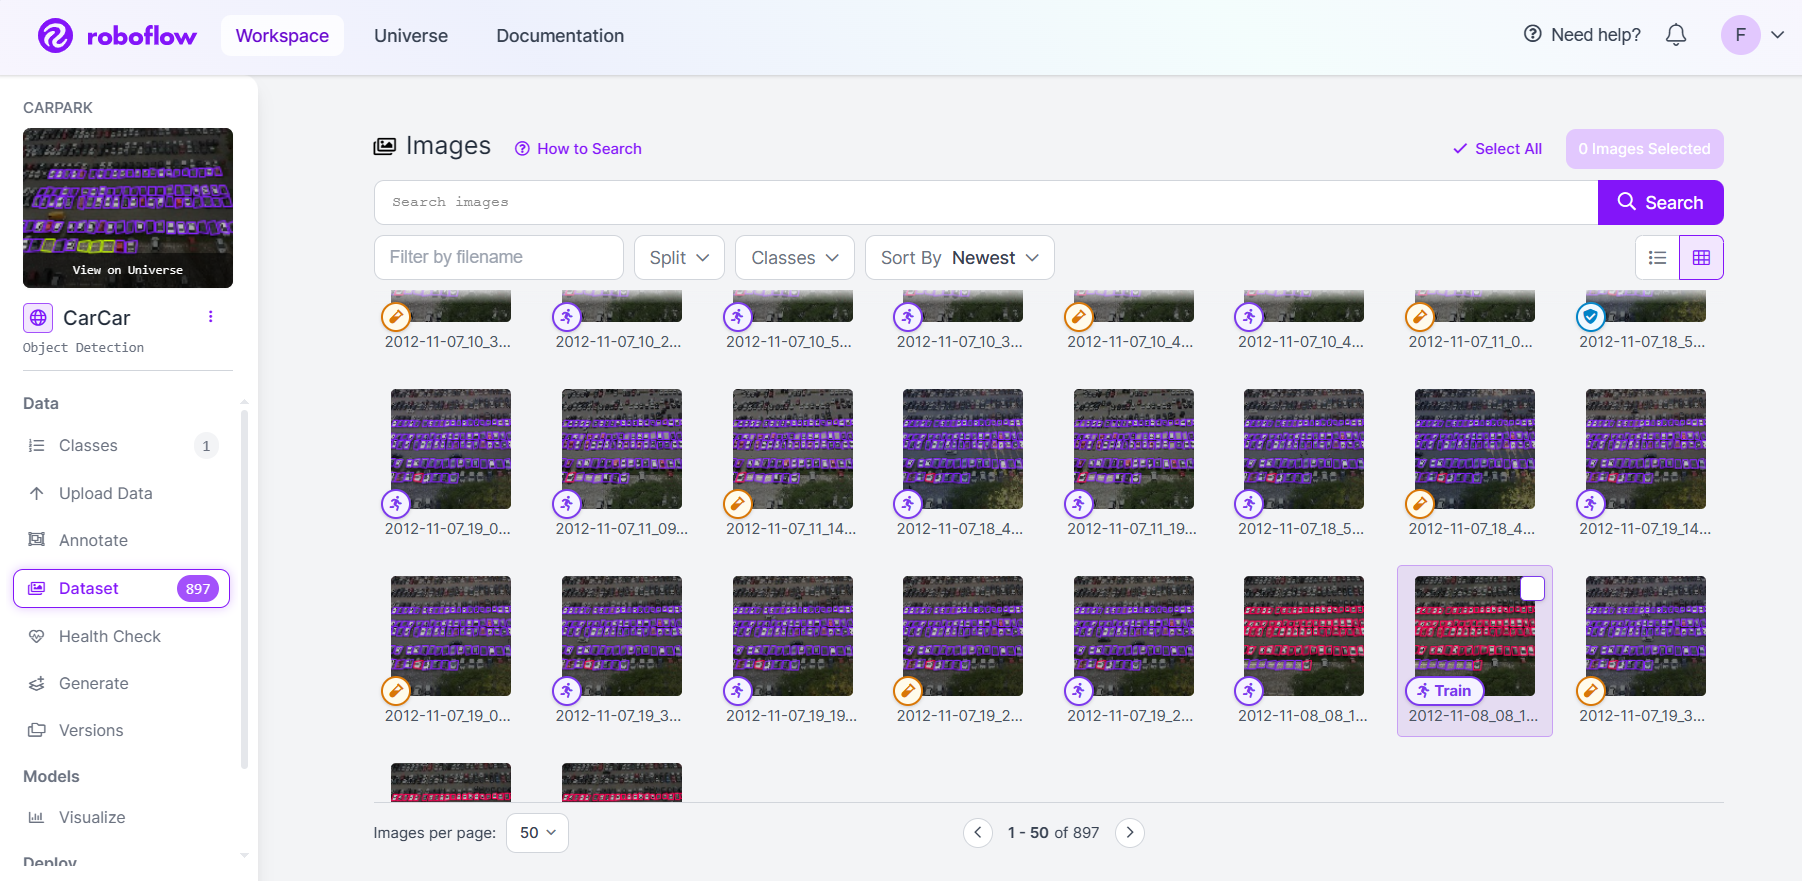
\includegraphics[ width=\textwidth]{roboflow.png}
   		\caption{Roboflow}
   	\end{figure}
   	\newpage
   	Görüntü etiketleme, bilgisayarlı görü (Computer Vision) modellerinin geliştirilmesinde çok önemli bir adımdır. Görüntü etiketleme, görüntülerin bilgisayarlı görü algoritmaları tarafından daha kolay anlaşılmasını sağlamak için bir görüntüye ilgili bilgilerin eklenmesidir. Etiketleme aşamasında sınırlayıcı kutular ve hatta görüntüdeki farklı nesnelerin ayrıntılı segmentasyonları yer alabilir.
   	\newline
   	
   	\begin{figure}[!h]
   		\centering
   		\includegraphics[ width=\textwidth]{etiket_ornek.png}
   		\caption{Roboflow : Etiketlemeye örnek}
        \label{etiket}
   	\end{figure}
   	
   	\begin{figure}[!h]
   		\centering
   		\includegraphics[ width=\textwidth]{etiketli-veriler.png}
   		\label{ornek}
   		\caption{Roboflow}
   	\end{figure}
   	Şekil \ref{etiket} de etiketleme işlemine örnek verilmiştir.
   	
   	\newpage
   	\subsection{YOLO}
   	\begin{justify}
   	YOLO (You only look once) türkçe karşılığı ‘Yalnızca bir kez bak ‘ olan, gerçek zamanlı nesne takibi için CNN (Convolutional Neural Network -Evrişimli Sinir Ağı) kullanan en yaygın algoritmadır.Gerçek zamanlı nesne takibi için RCNN (Regions with Convolutional Neural Networks), Fast R CNN (daha hızlı ve daha verimli) , Faster R CNN (daha hızlı daha doğru sonuç- nesne tespiti ve bölge önerisi (region proposal) aşamalarını tek bir ağ içinde birleştirir.) gibi uygulamalar 2015 yılında YOLO piyasaya sürülene kadar kullanılan popüler uygulamalardı. YOLO’yu diğer uygulamalardan ayıran en önemli özelliği çok hızlı olmasıdır. YOLO’nun çalışma mekanizmasına bakıldığında diğer nesne algılama yöntemlerinden farklı ve hızlı kılan birçok yönü bulunmaktadır. 
   	\newline
   	
   	YOLO,görseli tek seferde bir sinir ağından geçirerek resimdeki nesnelerin koordinatlarını ve sınıfını tahmin eder. Bu, ağın bir resmi tek bir geçişte tarayarak ağır hesaplamalara gerek kalmadan nesneleri tespit edebilmesini sağlar. Bu tanımlamayı yaparken görseli 3*3 , 4*4,19*19 ızgaralara (grids) ayırır. Izgaraların sayısını belirlemek için belirli bir koşul yoktur. N*N formatında olması yeterlidir .Her ızgara kendi içerisinde nesne olup olmadığını ve nesne var olduğunu düşünüyorsa merkez noktasının kendi alanında olup olmadığını düşünür. Resim sinir ağından geçtikten sonra çıktı olarak bir vektör meydana gelir.\cite{mediumcom}
   	\end{justify}
   \clearpage
   	\begin{figure}[!h]
   		\centering
   		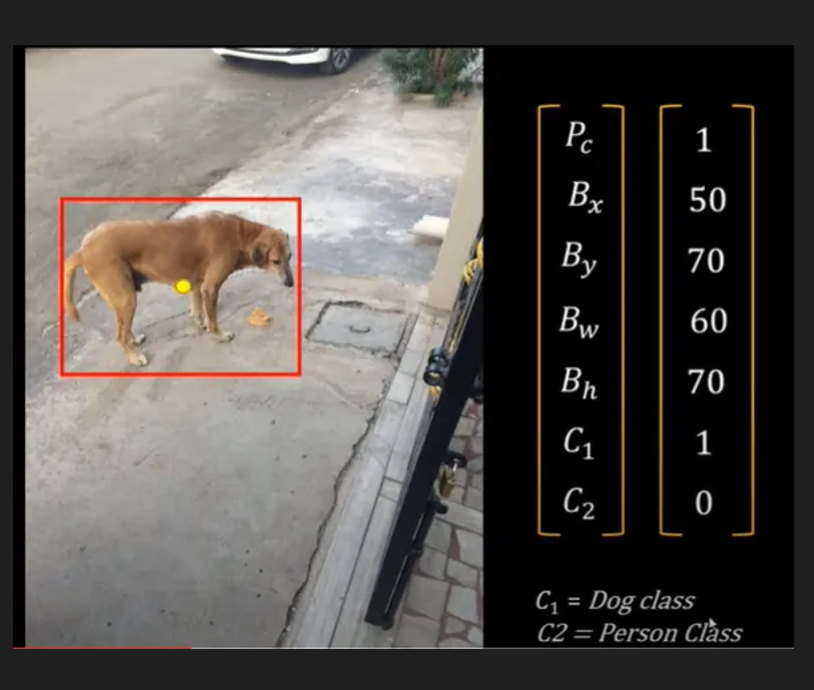
\includegraphics[ width=\textwidth]{matris.png}
   		\caption{Photo on Codebasics Youtube Channel by Dhaval Pate}
   		\label{fig:ornek}
   	\end{figure}
   	Şekil \ref{fig:ornek}'de görüldüğü gibi bir nesne için bir vektör meydana gelmektedir.
   	
   		\begin{itemize}
   		\item Pc (Probability of class): Sınıf olasılığıdır. Burada nesnenin yer alıp almamasına göre değerlendirme yapılır. Nesne olma olasılığı 1 ile , nesne olmama olasılığı 0 ile belli edilir. Bu görselde çerçevenin içerisinde köpek olduğu için Pc değeri 1'dir.
   		
   		\item  Bx: Köpeğin merkez noktasının (sarı nokta ile gösterilmiştir) x koordinatıdır.
   		
   		\item  By: Köpeğin merkez noktasının (sarı nokta ile gösterilmiştir) y koordinatıdır.
   		
   		\item  Bw: Kırmızı çerçevenin enidir .(Nesnenin eni, buradaki nesne köpektir.)
   		
   		\item Bh: Kırmızı çerçevenin yüksekliğidir. (Nesnenin yüksekliğidir, buradaki nesne köpektir.)
   		
   		\item  C1: Köpek sınıfını ifade eder.
   		
   		\item  C2: İnsan sınıfını ifade eder.
   		
   	\end{itemize} 
     
   	Nesne tespitine iki ana yaklaşım vardır:
   	\begin{itemize}
   		\item  İki aşamalı dedektörler Daha Hızlı R-CNN gibi, önce bölge önerileri üretir, ardından her bölgenin sınırlarını sınıflandırır ve hassaslaştırır. Daha doğru olma eğilimindedirler ancak daha yavaştırlar.
   		\item  Tek aşamalı dedektörler YOLO gibi, tek geçişte doğrudan görüntünün üzerine bir model uygulayın. Çok hızlı çıkarım süreleri için doğruluktan ödün veriyorlar.
   	\end{itemize}
   	
   	\begin{figure}[!h]
   		\centering
   		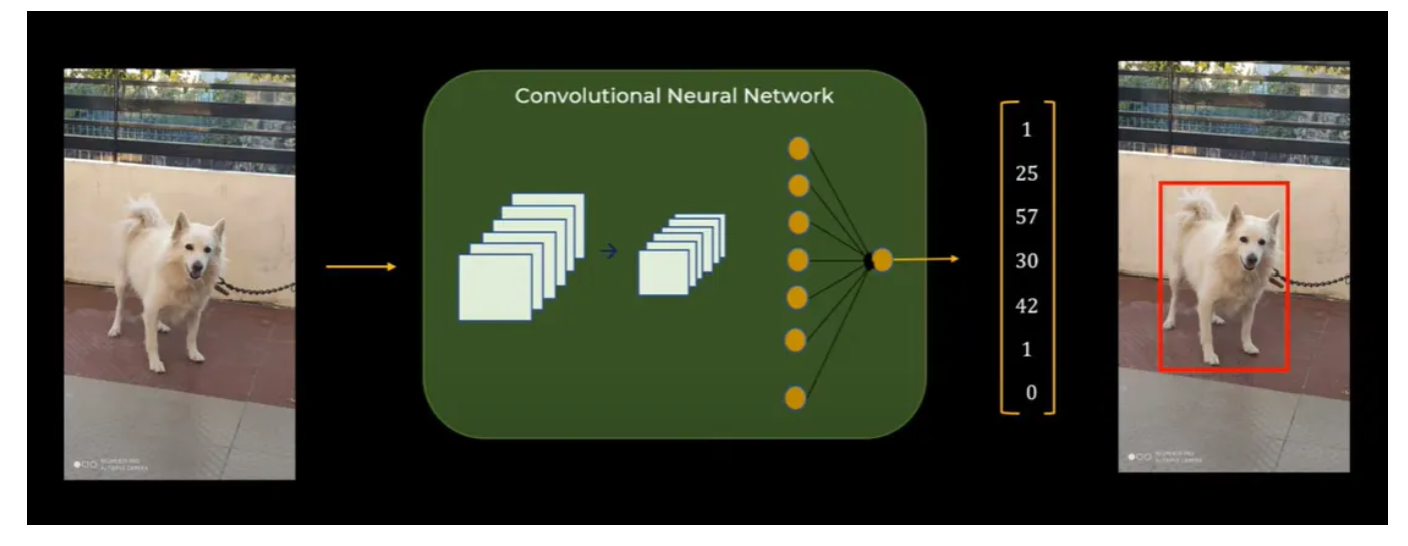
\includegraphics[width=\textwidth]{yolo}
   		\caption{Photo on Codebasics Youtube Channel by Dhaval Pate}
   		\label{fig:ornek2}
   	\end{figure}
   
   	
   	\begin{figure}[!h]
   		\centering
   		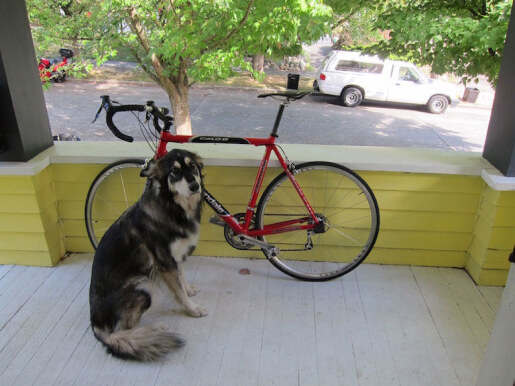
\includegraphics[width=0.7\textwidth]{nesnetanıma1}
   		\caption{Nesne tanıma işlemi yapılacak fotoğraf}
   		\label{fig:ornek3}
   	\end{figure}
   	
   	Şekil \ref{fig:ornek3}'deki resime YOLO ile nesne tanıma yaptırılacaktır. 
   	
   	
   	\begin{figure}[!h]
   		\centering
   		\includegraphics[ width=1.30\textwidth]{nesne tanıma2}
   		\label{ornek4}
   		\caption{detection işlemi yapılacak fotoğraf}
   	\end{figure}
   	\newpage
   	İlk önce girdi resmini SxS‘lik ızgaralara bölüyor.Her bir ızgara kendi içinde, alanda nesnenin olup olmadığını, varsa orta noktasının içinde olup olmadığını, orta noktası da içindeyse uzunluğunu, yüksekliğini ve hangi sınıftan olduğunu bulmakla sorumlu. Resimde köpeğin orta noktasının olduğu ızgara köpeğin tespit edilmesinden/etrafına kutucuk çizmesinden sorumlu.
   	\newline
   	
   	Buna göre YOLO her ızgara için ayrı bir tahmin vektörü oluşturur.Her bir ızgara sadece 1 tane nesne tanımlayabiliyor. \newline
   	
   	\textbf{Güven skoru:} Bu skor modelin geçerli ızgara içinde nesne bulunup bulunmadığından ne kadar emin olduğunu gösterir. (0 ise kesinlikle yok 1 ise kesinlikle var) Eğer nesne olduğunu düşünürse de bu nesnenin gerçekten o nesne olup olmadığından ve etrafındaki kutunun koordinatlarından ne kadar emin olduğunu gösterir.
   	\newline
   	
   	$ \text{Güven Skoru} = \text{Pr(obj)} \times \text{IoU} $
   	\newline
   	
   	Pr(obj): ızgara içinde nesnenin bulunma olasılığı
   	
   	IoU: gerçekte nesnenin bulunduğu kutu ile tahmin edilen kutunun kesişimi
   	\newline
   	
   	YOLO’nun çalışma mantığını özetlersek,
   	\begin{itemize}
   		\item Algoritma görseli öncelikle ızgaralara ayırır.
   		
   		\item Her bir bölgedeki nesnelerin etrafına çerçeve (bounding box) çizer.
   		
   		\item Her bir bölgede nesne bulunma olasılığını hesaplar.
   		
   		\item Her bir çerçeve (bounding box) için güven skoru hesaplar.
   	\end{itemize}
   	Diğer geleneksel nesne algılama yöntemlerine kıyasla YOLO, oldukça hızlı ve gerçek zamanlı uygulamalarda etkili bir şekilde çalışabilir. Bu özelliği, özellikle canlı video akışı gibi anlık işlemlerde ve gerçek zamanlı uygulamalarda avantaj sağlar.
   	
   	\begin{figure}[!h]
   		\centering
   		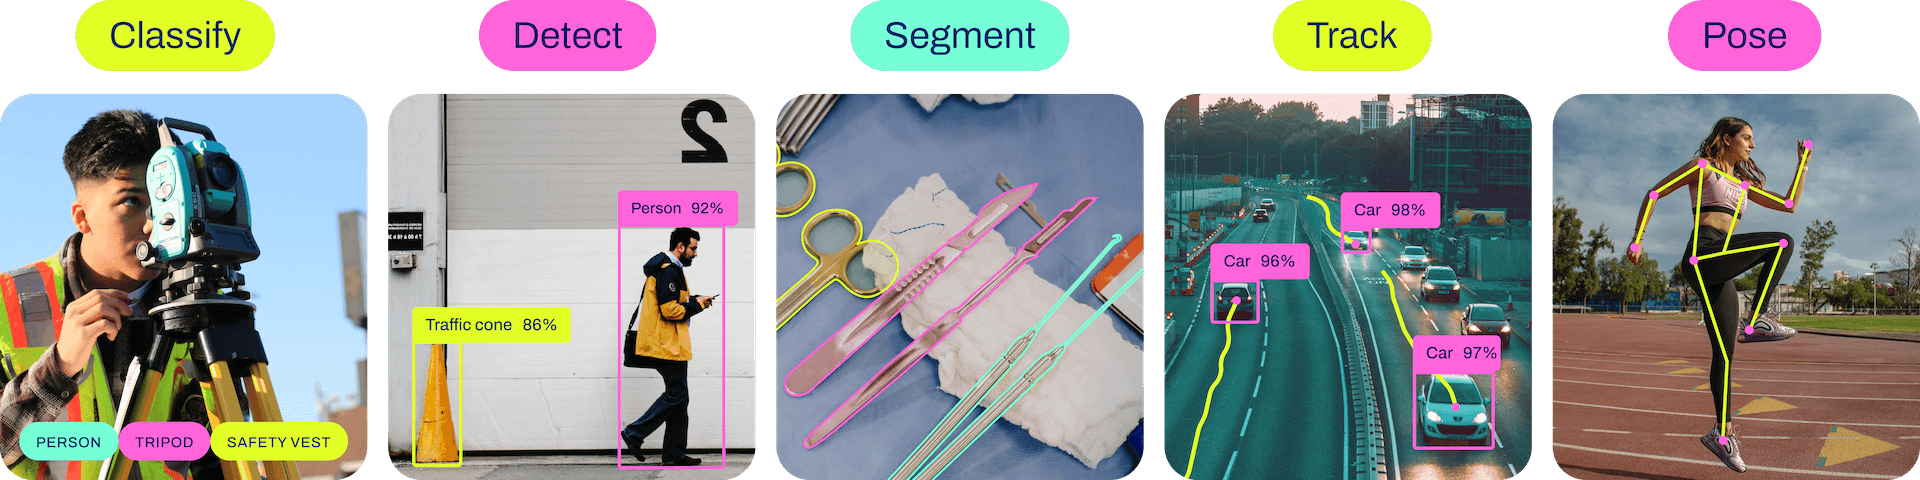
\includegraphics[width=\textwidth]{banner-tasks}
   		\caption{ultralytics}
   		\label{fig:ornek5}
   	\end{figure}
   	\subsubsection{Detection (COCO)}
   	
   	COCO, nesne tanıma, nesne tespiti ve nesne segmentasyonu için popüler bir veri kümesidir. İçinde 80 farklı nesne kategorisi barındırır ve her bir resimde bu nesnelerin detaylı etiketleri bulunur. Özellikle nesne segmentasyonu için ayrıntılı piksel bazında segmentasyon maskeleri sağlar.
   	
   	\subsubsection{Detection (Open Image V7)}
   	
   	Google tarafından sunulan büyük bir resim veri kümesidir. COCO'dan daha geniş bir etiket kategorisi yelpazesi sunar ve 9 milyondan fazla etiketlenmiş resme sahiptir. Sınırlayıcı kutular ve sınıf etiketleriyle nesne tespiti ve sınıflandırma görevlerinde kullanılır.Open Images, COCO gibi ayrıntılı piksel bazında segmentasyon maskeleri sağlamaz. Ancak nesnelerin sınırlayıcı kutuları ve sınıf etiketleri mevcuttur.
   	\newline
   	
   	\textbf{ Farkları}
   	\newline
   	
   	COCO, daha az etiket kategorisine sahip olmasına rağmen, nesne segmentasyonu için detaylı maske bilgileri sağlar.
   	Open Images V7, çok daha geniş bir etiket kategorisi yelpazesi sunar ve çok daha fazla sayıda resme sahiptir.
   	COCO'nun daha spesifik görevler için daha ayrıntılı veri sağladığı söylenebilirken, Open Images V7 daha genel ve çeşitli veri sağlar.
   	Hangi veri kümesinin kullanılacağı, kullanım senaryosuna ve ihtiyaca bağlıdır. Örneğin, daha geniş bir nesne kategorisi yelpazesi gerekiyorsa Open Images V7 tercih edilebilirken, nesne segmentasyonu gibi piksel bazında ayrıntılı bilgiler gerekiyorsa COCO daha uygun olabilir.\cite{ultralytics}
   	\newpage
   	
   	\subsubsection{Segmentation}
   	Temelde, bir görüntüdeki nesnelerin veya bölümlerin (segmentlerin) belirlenmesi işlemidir. Bu işlem, görüntüdeki pikselleri farklı nesnelere veya bölümlere ayrılmış gruplara ayırarak gerçekleştirilir. Segmentasyon, nesne tanıma, nesne tespiti, nesne izleme, medikal görüntüleme ve daha birçok alanda kullanılır.
   	
   	\begin{figure}[!h]
   		\centering
   		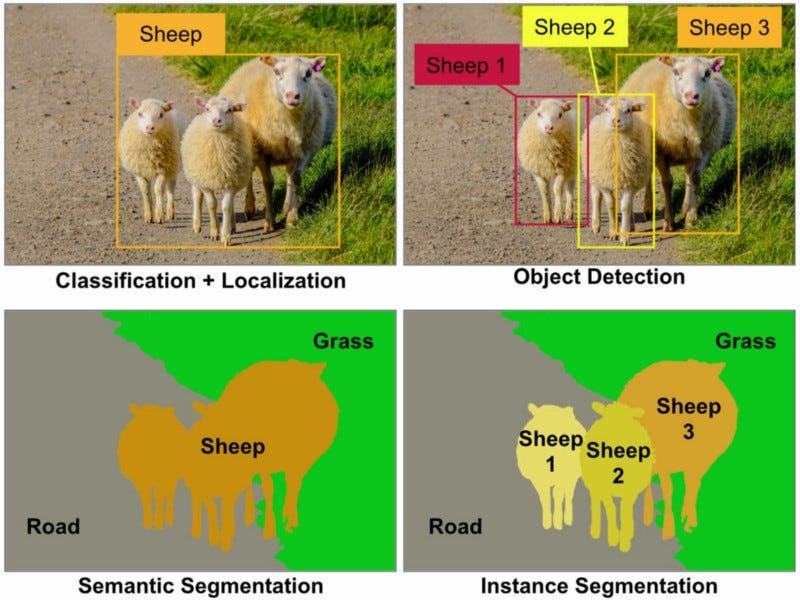
\includegraphics[width=\textwidth]{segmentation-1}
   		\caption{segmentation}
   		\label{fig:ornek6}
   	\end{figure}
   	
   	\textbf{Semantic (Anlamsal) Segmentasyon:} "Semantic Segmentasyon" veya "Anlamsal Segmentasyon", bir görüntüdeki her bir pikselin ait olduğu nesne veya bölge sınıfını belirlemeyi amaçlayan bir görüntü işleme ve derin öğrenme görevidir. Temel amacı, görüntüdeki her pikseli, o pikselin ait olduğu nesne veya bölgenin genel sınıfına atamaktır. Bu yöntem, pikselleri ayrı ayrı nesnelere veya bölümlere sınıflandırarak görüntüyü anlamlandırmayı hedefler.
   	\newline
   	
   	\textbf{Instance Segmentation:}nesne algılama ve nesne segmentasyonu yöntemlerinin bir kombinasyonudur.Bu yöntem, bir görüntüdeki her bir nesneyi ayrı tanımlamayı ve sınıflandırmayı, aynı zamanda her bir nesnenin piksel bazında segmentasyonunu gerçekleştirmeyi amaçlar. Yani, görüntüdeki her bir nesneyi belirlerken, nesnelerin sınırlarını (bounding box) çizerken aynı zamanda her bir nesnenin piksellerini de ayrı tanımlar.
   	
   	\subsubsection{Classification}
   	
   	"Classification" (Sınıflandırma), makine öğrenimi ve derin öğrenme alanlarında önemli bir konsepttir. Temelde, bir girdiyi belirli bir kategoriye veya sınıfa atama işlemidir. Bu işlem genellikle önceden belirlenmiş bir sınıf listesinden birine karar vermek için yapılır. Örneğin, bir resmi "köpek", "kedi", "araba" gibi belirli bir kategoriye sınıflandırmak gibi.\cite{Segmentasyon}
   	
   	\begin{figure}[!h]
   		\centering
   		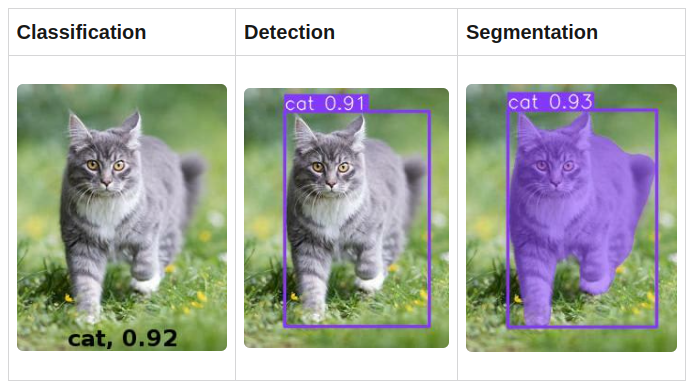
\includegraphics[width=\textwidth]{compvision}
   		\caption{segmentation}
   		\label{fig:ornek7}
   	\end{figure}
   \end{justify}
   
   \subsection{OPENCV}
   \begin{justify}
   OpenCV, çeşitli formatlardaki görüntüleri ve videoları yüklemek, görüntülemek ve kaydetmek için kolay kullanımlı fonksiyonlar sağlamaktadır.Görüntülerin ve videoların keskinleştirilmesi, bulanıklaştırılması, gri tonlamaya dönüştürülmesi gibi çeşitli ön işleme adımlarını gerçekleştirmektedir. OpenCV, derin öğrenme modellerini (örneğin, YOLO, SSD, Faster R-CNN) kullanarak nesne tanıma gerçekleştirmek için DNN (Deep Neural Network) modülünü içermektedir.
   \newline
   
   OpenCV, gerçek zamanlı video akışını (örneğin, bir web kamerasından gelen video) işleyebilmekte ve bu akış üzerinde nesne tanıma algoritmalarını çalıştırabilmektedir.Hareketli nesnelerin algılanması ve izlenmesi için kullanılabilmektedir.Nesnelerin daha hassas bir şekilde tanımlanması için görüntü segmentasyonu teknikleri kullanılmaktadır.Bu projede OpenCV, kendi verilerimizi kullanarak makine öğrenimi modelleri eğitmek ve bu modelleri nesne tanıma için kullanmak için araçlar sağlamaktadır.
   \subsubsection{OpenCV’de Canny Fonksiyonu ile Kenar Tespiti}
   
   Canny kenar tespit fonksiyonu, eşik değerleri arasındaki piksel değerlerini kullanarak görüntüdeki kenarları tespit eder.Görüntü parlaklığının keskin bir şekilde değiştiği noktaları tespit etmeye dayanan bir algoritmadır.
   \begin{itemize}
   	\item Threshold1: Minimum eşik değeri. Bu değer altındaki piksel değerleri kenar olarak tanımlanmaz.(Düşük eşik değeri, daha fazla gürültü ve fazla sayıda kenar tespiti anlamına gelir.)
   	\item Threshold2 : Maksimum eşik değeri. Bu değer üzerindeki piksel değerleri kenar olarak tanımlanır.(Yüksek eşik değeri, daha az gürültü ve daha az sayıda kenar tespiti anlamına gelir.)\newline
   \end{itemize}
   
   	Canny kenar tespiti fonksiyonunun minimum eşik değeri “0” ve maksimum eşik değeri “255” olarak ayarlanmıştır.Eşik değerleri arasındaki piksel değerleri, görüntüdeki kenarları tanımlamak için kullanılır ve sonuç binary bir görüntü olarak döndürülür.
   \newline
   
   Threshold1 ve Threshold2 değerlerinin seçimi kullanılan görüntüye göre değişkenlik gösterir. Canny fonksiyonunu kullanmadan önce görüntüye bazı filtreler uygulanabilir.
   
   
   
   
   \subsubsection{Adım 1: Görüntünün Yüklenmesi ve Ölçeklendirilmesi}
   İlk adımda, bir görüntü yüklenir ve isteğe bağlı olarak belirtilen bir ölçekte yeniden boyutlandırılır. Ölçeklendirme, görüntünün işlem süresini azaltmak ve bellek kullanımını kontrol etmek için kullanışlıdır. Örneğin, büyük bir görüntüyü işlerken bilgisayar kaynaklarına daha az yük bindirmek için ölçeklendirme yapılabilir.
   
   \subsubsection{Adım 2: Önişleme (Preprocessing)}
   Önişleme adımı, görüntü üzerinde bazı ön işlemlerin gerçekleştirildiği aşamadır. Bu adımlar şunları içerir:
   \begin{itemize}
   	\item Gri Tonlama (Grayscale): Renkli bir görüntüyü gri tonlamaya dönüştürmek, işlemleri basitleştirmek için yaygın bir adımdır. Gri tonlamalı görüntü, her pikseldeki renk bilgisini tek bir yoğunluk değerinde temsil eder.
   	
   	\item Gaussian Bulanıklaştırma (Gaussian Blur): Gürültüyü azaltmak ve daha iyi kenar algılaması için görüntüye bir Gaussian filtresi uygulanır. Bu, kenarların daha belirgin olmasını sağlar.
   	
   	\item Kenar Algılama (Canny Edge Detection): Kenar algılama, görüntüdeki önemli kenarları tespit etmek için kullanılır. Canny kenar algılama, diğer yöntemlere göre daha hassas ve doğru sonuçlar verir.
   	
   	\item Morfolojik İşlemler (Dilation ve Closing): Dilation, kenarların kalınlığını artırarak görüntüdeki boşlukları doldurur. Closing, kenarları birleştirerek nesnelerin daha düzgün bir şekilde algılanmasını sağlar.
   \end{itemize}
   
   \subsubsection{Adım 3: Kontur Bulma ve Köşe Noktalarının Tespiti}
   Kontur bulma, görüntüdeki nesnelerin sınırlarını belirlemek için kullanılır. Burada, nesnenin dış sınırlarını çevreleyen bir kontur elde edilir. Bu kontur, nesnenin şeklini ve boyutunu belirlemek için kullanılacaktır.
   
   Kontur tespiti yapıldıktan sonra, nesnenin köşe noktalarını tespit etmek için bir dizi işlem yapılır. Bu köşe noktaları, nesnenin dörtgen bir şekil olduğunu düşünerek, daha sonra perspektif dönüşümü için kullanılacaktır.
   
   \subsubsection{Adım 4: Perspektif Dönüşümü (Warping)}
   Perspektif dönüşümü adımında, nesnenin görsel olarak düz bir açıdan görülebilmesi için görüntü üzerinde bir dönüşüm yapılır. Bu adım, nesnenin gerçek boyutunu doğru bir şekilde belirleyebilmek için önemlidir. Örneğin, bir A4 kağıdının köşe noktaları belirlenerek bu köşe noktalarından bir dörtgen oluşturulur ve bu dörtgen, görüntüdeki nesnenin yerini temsil eder. Daha sonra bu dörtgen, A4 kağıdının gerçek boyutlarına göre yeniden boyutlandırılır.
   
   \subsubsection{Adım 5: Boyutların Hesaplanması}
   Perspektif dönüşümü sonrasında, dönüştürülen nesnenin genişliği ve yüksekliği piksel cinsinden hesaplanır. Bu adım, nesnenin görüntü üzerindeki piksel boyutlarını belirler.
   \newline
   
   \subsubsection{Adım 6: Piksel Boyutlarının Gerçek Boyutlara Dönüştürülmesi}
   Son olarak, nesnenin piksel boyutları gerçek dünya boyutlarına dönüştürülür. Bu adım, bir referans nesne kullanarak gerçek dünya boyutlarına göre piksel boyutlarının hesaplanmasını içerir. Örneğin, bir A4 kağıdının gerçek boyutlarını biliyorsak ve görüntüdeki A4 kağıdının piksel boyutlarını hesapladıysak, diğer nesnelerin boyutlarını da bu oranlar kullanılarak hesaplayabiliriz.
   \newline
   
   Bu adımlar, nesnenin boyutunu belirlemek için tipik olarak izlenen adımlardır ve bu sürecin bir parçası olarak siyah-beyaz yapma, kenar algılama, kontur bulma ve perspektif dönüşüm gibi işlemler kullanılır. Bu işlemler, nesnenin görüntü üzerindeki belirginliğini artırarak ve perspektif etkisini düzelterek doğru boyutları elde etmeyi sağlar.\cite{Nesne-Boyutunu-Bulma-Adımları}
   \newpage
   \end{justify}
   
  \subsection{MEDİAPİPE}
  \begin{figure}[!h]
  	\centering
  	\includegraphics[width=0.8\textwidth]{mediapipe-el}
  	\caption{MediaPipe-El Eklemleri}
  
  \end{figure}
 \begin{justify}
 	 Meyve ve sebzelerin gerçek boyutlarını belirlemek için el ve tırnak boyutunu referans alacak. Kameradan alınan görüntülerle el ve tırnak boyutları ölçülerek meyvelerin gerçek boyutları hesaplanacaktır.
 	Kameradan alınan görüntülerle elin boyutları ölçülecektir. En geniş, en uzun ve en dar noktaların ölçüleri kaydedilecektir.Tırnak boyutları, işaret, orta, yüzük, serçe ve küçük parmakların tırnaklarından ayrı ayrı ölçülecektir. Her bir parmak için tırnak uzunluğu belirlenecektir.\newline
 	
 	Mediapipe ve OpenCV gibi görüntü işleme kütüphaneleri kullanılarak, kameradan alınan görüntülerde el ve tırnaklar tanımlanacaktır. Bu adımda, elin genel yapısı ve tırnakların konumu tespit edilecektir.El ve tırnak boyutları piksel cinsinden ölçüldükten sonra, kameranın sabit bir uzaklığına göre gerçek dünya ölçülerine dönüştürülecektir.El ve tırnak boyutları referans alınarak, meyve ve sebzelerin görüntülerinde el ile karşılaştırma yapılacaktır.El ve tırnak boyutlarına göre meyve ve sebzelerin gerçek boyutları hesaplanacaktır.\footnote{Bu yöntem, meyve ve sebzelerin gerçek boyutlarını belirlemek için kullanılan bir referans ölçüm yöntemidir.}
 	 \begin{figure}[!h]
 		\centering
 		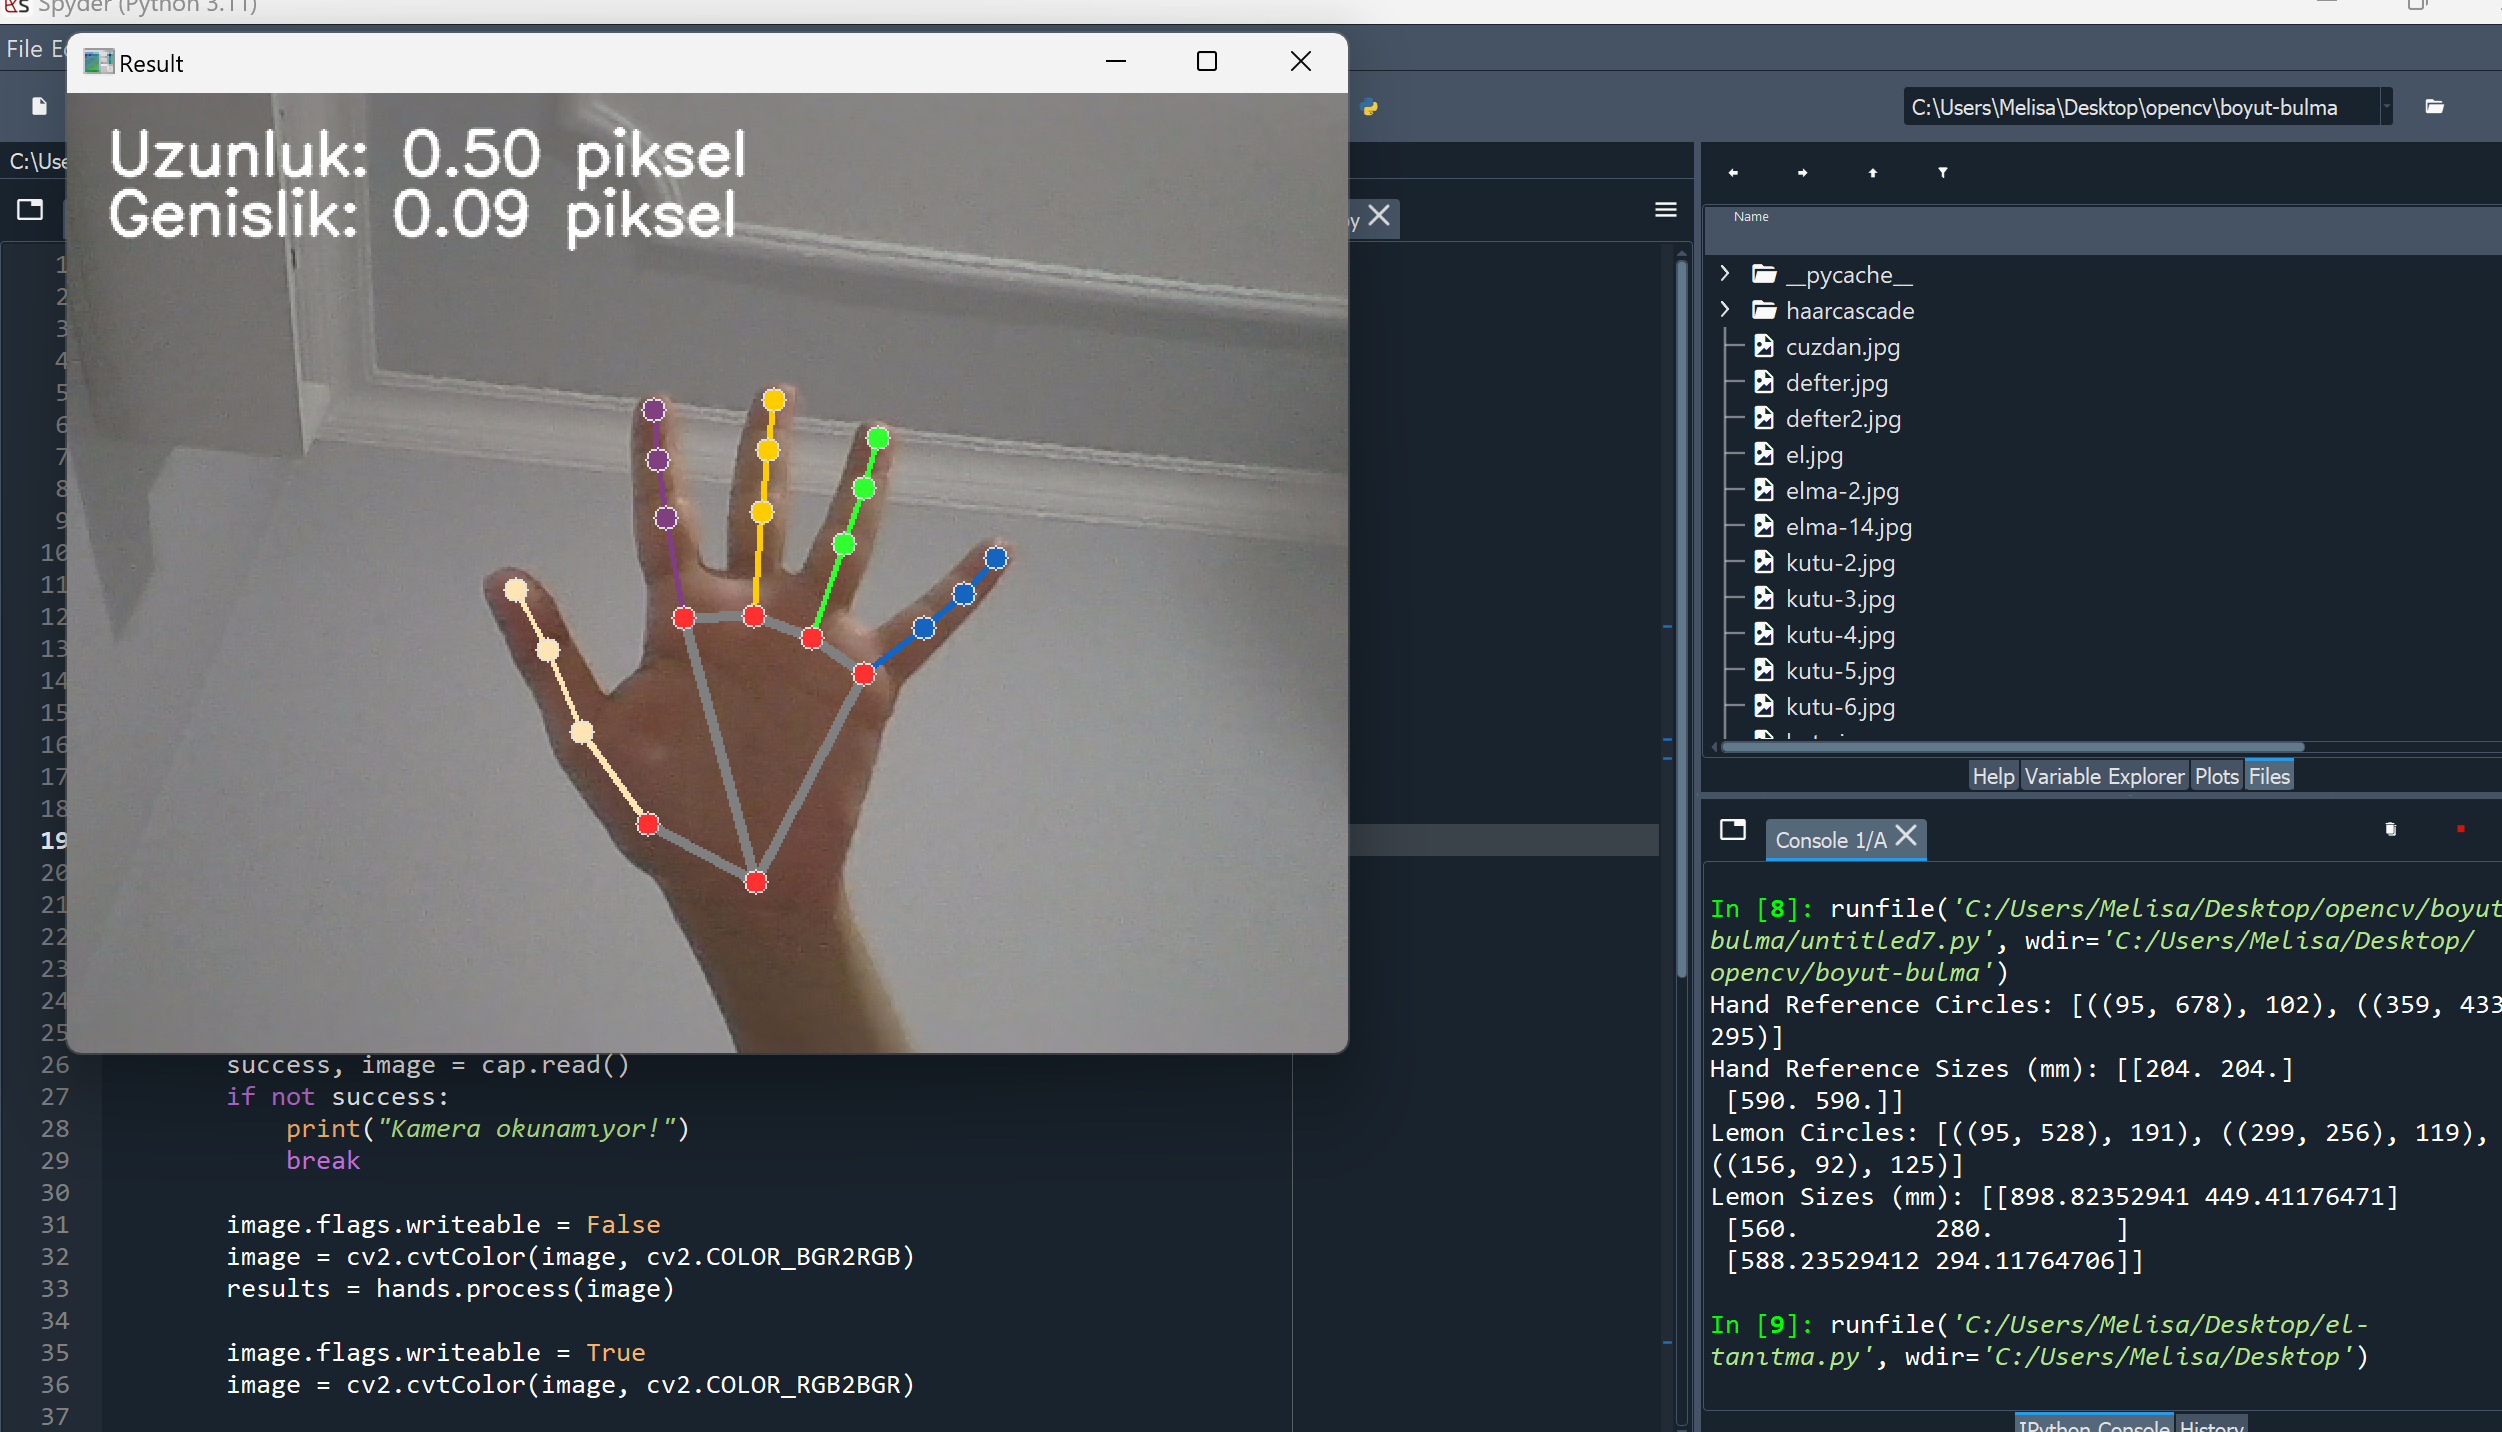
\includegraphics[width=0.4\textwidth]{el-boyut}
 		\caption{MediaPipe Webcamden El Tespiti}
 		
 	\end{figure}
 	\clearpage
 	\subsection{Antropometri Nedir?}
 		Antropometri tanımı, “insan” ve “ölçüm” anlamına gelen antropos ve metrikos Yunanca kelimelerine dayanmaktadır. İlgili alanlarda kullanılmak üzere insan vücudu parçalarının ölçüm verilerini organize etme, türetme ve analiz etme bilimidir.
 		Antropometri, bireysel farklılıklara odaklanan ve çeşitli tasarım disiplinleri için önemli referanslar ve girdiler sağlayan ergonomi uygulamalarının hayati bir parçasıdır.Koltuklar, konsollar, ATM, araç iç hacimleri, cep telefonları, gamepadlar gibi insan vücudu ölçüleri içeren ürünler için ana tasarım çalışma konularından biridir. Mekanik tasarım yapacak mühendisler için de antropometri çalışmaları zaman zaman önem kazanmaktadır.\cite{antropometrinedir}
 		
 		Vücut ölçülerinin elde edilmesine yönelik, statik ve dinamik (fonksiyonel) antropometri olmak üzere iki farklı metot geliştirilmiştir.
 		
 		\subsubsection{Statik antropometri}İnsanların statik duruş ve oturuşlarında ölçülen boyutları ele alan bir uğraş alanıdır. Antropometrik ölçüler ayakta durma ve düz bir zeminde oturma durumlarına bağlı olarak özel aletlerin kullanımıyla alınmakta ve farklı ergonomik tasarımlarda kullanılmaktadır.Statik boyutlar, dirsek ve bilek arası ölçümler ile eklem merkezleri arasında ölçümler gibi insan iskeleti boyutları yanı sıra baş çevresi, cilt yüzeyi çevre ölçüleri gibi dış hat boyutlarını içermektedir.Çeşitli yaş gruplarındaki okul çocuklarının oturacağı sıraların boyutlarını saptamanın yanı sıra, bir gaz maskesinin yüz ölçülerine uygun bir şekilde ve boyutlarda imali için ihtiyaç duyulan antropometri ölçümler de statik antropometri yaklaşımı ile elde edilir.
 		\subsubsection{Dinamik Antropometri}
 		Endüstri ve iş ortamında iş görenler sürekli devinim hâlindedirler. Bir iş gören işini yaparken çeşitli yönlere uzanması, kol, bacak ve gövdesini değişik boyutlarda ve devamlı hareket ettirmesi nedeni ile çeşitli dinamik ölçülerin bilinmesine ihtiyaç duyulur. Fonksiyonel antropometri olarak da bilinen dinamik antropometri yaklaşımı ile elde edilen boyutlar, bazı fiziksel aktivitelerde bulunan insan vücudundan belli şartlar altında elde edilirler. İnsanların ayakta dururken ya da otururken çevrelerindeki malzemelere, kontrol sistemlerine ve çeşitli işlem noktalarına uzanabilmeleri için; eğilme, uzanma ve dönme gibi hareketlerinin hudutlarını ölçmek de iş düzeni ve insan-tezgâh, insan-makine gibi arakesitlerin tasarımında optimizasyon açısından önemlidir. Ancak çalışma ortamında insanların, sekreterin masasında bulunan telefona erişmesi, masanın çekmecesinden kâğıt almak için eğilmesi örneklerinde olduğu gibi, hareketlerde bulunmaları nedeniyle çeşitli dinamik boyutların ölçülmesine ihtiyaç duyulmuştur. İnsanların ayakta dururken ya da otururken çevrelerindeki malzemelere, kontrol araçlarına ve çeşitli işlem noktalarına eğilme, dönme, uzanma gibi hareketlerle erişebilecekleri sınırlar dinamik antropometri ile ölçülür.
 		
 		
 		\subsubsection{Insan Bedeninde Altın Oran}
 		
 		İnsan vücudunda altın orana verilebilecek ilk örnek, göbek ile ayak arasındaki mesafe bir birim olarak kabul edildiğinde, insan boyunun $1,618'$e denk gelmesidir. Bunun dışında vücudumuzda yer alan diğer bazı altın oranlar şöyledir:
 		
 		\begin{itemize}
 			\item Parmak ucu ile dirsek arası / El bileği ile dirsek arası
 			\item Omuz hizasından başucuna olan mesafe / Kafa boyu
 			\item Göbek ile başucu arası mesafe / Omuz hizasından başucuna olan mesafe
 			\item Göbek ile diz arası / Diz ile ayakucu arası mesafe
 		\end{itemize}
 		
 		Altın oran ile uyumlu tüm yapıların insan gözüne estetik açıdan ve uzunlukların birbirlerine uyumu açısından en güzel algılanan yapılar olduğu ve tercih sebebi olduğu gösterilmiştir. Altın oran parçalar veya uzuvlar arasında içsel bir uyum ve güzelliği bulundurur. Bu orana sahip bütünün tüm öğeleri insan gözüne çekici, estetik ve güzel gelmektedir. Altın orana diğer bir örnek ise Fibonacci dizisine tam bir uygunluk gösteren insan elidir. Parmaklarımız üç boğumludur. Parmağın tam boyunun ilk iki boğuma oranı altın oranı verir (başparmak dışındaki parmaklar için). Ayrıca orta parmağın serçe parmağına oranında da altın oran olduğunu fark edilebilmektedir.
 		
 		\begin{figure}[!h]
 			\centering
 			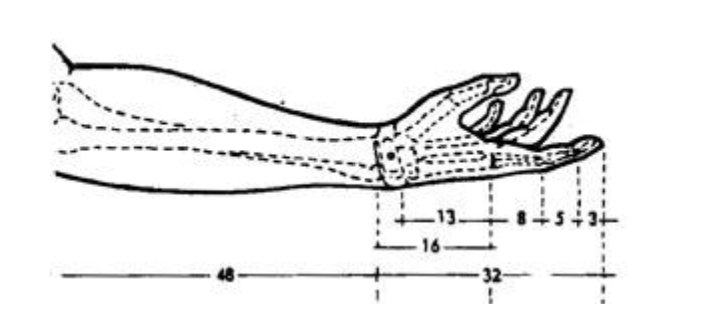
\includegraphics[ width=0.7\textwidth]{el}
 			\caption{Parmaktaki Altın Oran}
 			\label{el}
 		\end{figure}
 		
 		
 		
 		Şekil \ref{el} de her ardışık bölüm arasındaki oran altın oran sabiti olan $0,518\ldots$ sayısıdır. Ayrıca her bölüm 2, 3, 5, 8'e yani ardışık Fibonacci sayılarına karşılık gelmektedir.
 		
  \subsection{DATA AUGMENTATİON - VERİ ARTTIRMA}
 		Veri artırma, uygulayıcıların, aslında yeni veriler toplamadan, eğitim modelleri için mevcut olan veri çeşitliliğini önemli ölçüde artırmasına olanak tanıyan bir stratejidir. Kırpma, doldurma ve yatay çevirme gibi veri artırma teknikleri, büyük sinir ağlarını eğitmek için yaygın olarak kullanılır \cite{Augmentation1}. 
 	\newline
 	
 	Bu teknik , makine öğrenimi modellerini eğitirken aşırı uyumu azaltmak için makine öğreniminde yaygın olarak kullanılır, modelleri biraz değiştirilmiş birkaç kopya üzerinde eğiterek elde edilir.Veri büyütme, model genellemesini ve performansını iyileştirmek için eğitim veri seti çeşitliliğini zenginleştirerek görüntü sınıflandırmada temel hale geldi . Bu uygulamanın gelişimi, geometrik dönüşümler, renk alanı ayarlamaları ve gürültü enjeksiyonu dahil olmak üzere geniş bir teknik yelpazesini ortaya çıkarmıştır.
 	
 	\subsection{Geometrik Dönüşümler }
 	Geometrik dönüşümler, farklı perspektifleri, yönelimleri ve ölçekleri simüle etmek için görüntülerin uzamsal özelliklerini değiştirir.
 	\newline
 	
 	Yaygın teknikler şunları içerir:
 	\newline
 	
 	\textbf{Döndürme:}Modellerin nesneleri çeşitli açılardan tanımasına yardımcı olmak için görüntüleri belirli bir dereceye kadar döndürme.\newline
 	
 	\textbf{Çevirme:} Yönlendirmede değişkenlik sağlamak için görüntüleri yatay veya dikey olarak yansıtmak.\newline
 	
 	\textbf{Kırpma:} Belirli özelliklere odaklanmak veya daha yakın görünümleri simüle etmek için görüntünün bazı bölümlerini kaldırmak.\newline
 	
 	\textbf{Çeviri:} Modellere konumsal değişmezliği öğretmek için görüntüleri farklı yönlere kaydırmak.
 	\newpage
 	
 	\subsection{Renk Uzayı Dönüşümleri }
 	Renk alanı dönüşümleri, aydınlatma, renk doygunluğu ve kontrasttaki farklılıklara değinerek görüntülerin renk özelliklerini değiştirir.\newline
 	
 	Teknikler şunları içerir:\newline
 	
 	\textbf{Parlaklık Ayarı:} Farklı aydınlatma koşullarını simüle etmek için görüntünün parlaklığını değiştirme.\newline
 	
 	\textbf{Kontrast Ayarı:} Modellerin çeşitli netlik seviyelerindeki nesneleri tanımasına yardımcı olmak için kontrastın değiştirilmesi.\newline
 	
 	\textbf{Doygunluk Ayarı:} Farklı renk yoğunluklarına sahip görüntülere yönelik modeller hazırlamak amacıyla doygunluğun değiştirilmesi.\newline
 	
 	\textbf{Renk Değişimi:} Renk değişkenliği sağlamak için parlaklık, kontrast, doygunluk ve renk tonunun rastgele ayarlanması \cite{Augmentation2}.
 	\begin{figure}[!h]
 		\centering
 		\includegraphics[ width=\textwidth]{augmentation1}
 		\caption{Augmentation \cite{Augmentation1}}
 		
 	\end{figure}
 	\clearpage
 
 	\section{Veri Çoğaltma}
 	\begin{figure}[!h]
 		\centering
 		\begin{minipage}[b]{0.48\textwidth}
 			\centering
 			\includegraphics[width=\textwidth]{orijinal}
 			\subcaption{Orijinal Görsel}
 		\end{minipage}
 		\hspace{0.04\textwidth}
 		\begin{minipage}[b]{0.48\textwidth}
 			\centering
 			\includegraphics[width=\textwidth]{contrast}
 			\subcaption{Contrast Uygulanmış Görsel}
 		\end{minipage}
 		\vspace{0.04\textwidth}
 		\begin{minipage}[b]{0.48\textwidth}
 			\centering
 			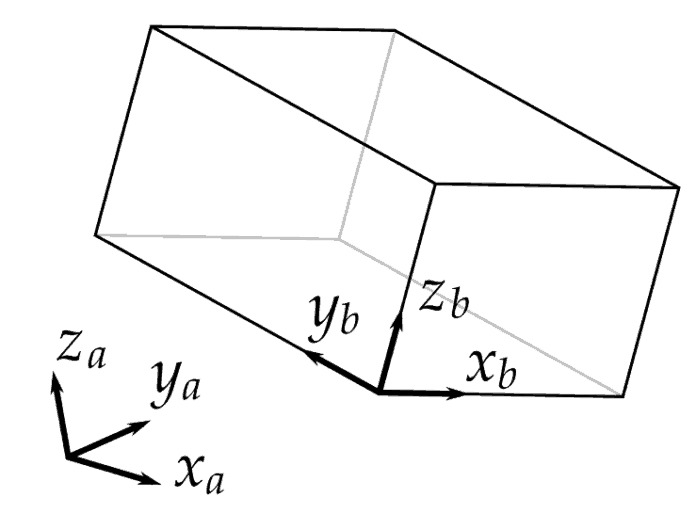
\includegraphics[width=\textwidth]{rotation}
 			\subcaption{Rotation Edilmiş Görsel}
 		\end{minipage}
 		\caption{Augmentation Örneği}
 	\end{figure}
 	\clearpage
 	\section{PIL Kütüphanesi}
 	Python Imaging Library (kısaca PIL), Python programlama dili için geliştirilen, açık kaynak kodlu grafik işleme kütüphanesidir. Bu kütüphane, içinde barındırdığı hazır fonksiyonlar sayesinde programcıya üstün bir grafik işleme imkânı sunar. Birçok grafik türünü açıp kaydetme yeteneği ile birlikte çizim, düzenleme, filtreleme gibi işlemlerde kullanılabilecek fonksiyonlara sahiptir\cite{PIL}.
 	\newline
 	
 	\section{Sequential Modeli:}
 	Sequential modeli, katmanları ardışık olarak ekleyerek oluşturulan bir model türüdür. Her bir katman, kendisinden önceki katmanın çıktısını girdi olarak alır.
 
 	\subsubsection{AUGMENTATİON KOD PARÇASI}
 	\begin{verbatim}
 		num_classes = 5
 		
 		model = Sequential([
 		data_augmentation,
 		layers.Conv2D(16, 3, padding='same', activation='relu'),
 		layers.MaxPooling2D(),
 		layers.Conv2D(32, 3, padding='same', activation='relu'),
 		layers.MaxPooling2D(),
 		layers.Conv2D(64, 3, padding='same', activation='relu'),
 		layers.MaxPooling2D(),
 		layers.Dropout(0.2),
 		layers.Flatten(),
 		layers.Dense(128, activation='relu'),
 		layers.Dense(num_classes)
 		])
 		
 		model.compile(optimizer='adam',
 		loss=tf.keras.losses.SparseCategoricalCrossentropy(from_logits=True),
 		metrics=['accuracy'])
 		
 		model.fit(X_train_scaled, y_train, epochs=30)
 	\end{verbatim}
 	\clearpage
 \begin{itemize}
 	
 	\subsubsection{AUGMENTATİON KODUNUN TERMİNOLOJİSİ}
 	\item  Sequential: Katmanları sırayla eklememizi sağlar.
 	\item   Conv2D: İki boyutlu konvolüsyon katmanıdır. Görüntü verilerini işlemede kullanılır.
 	\item   16, 32, 64: Filtre sayısını belirtir.
 	\item   3: Çekirdek boyutunu (3x3) belirtir.
 	\item   padding='same': Çıktının giriş ile aynı boyutta olmasını sağlar.
 	
 	\item   MaxPooling2D: Maksimum havuzlama katmanıdır. Uzaysal boyutları küçültmek için kullanılır.
 	
 	\item  Flatten: Çok boyutlu girişleri tek boyutlu vektöre dönüştürür.
 	
 	\item  Dense: Tam bağlantılı katmandır. Her nöron bir önceki katmandaki tüm nöronlara bağlıdır.
 	
 	\item  128: Nöron sayısını belirtir.
 	activation='relu': ReLU aktivasyon fonksiyonunu kullanır.\newline
 	
 	\item  model.fit(X-train-scaled, y-train, epochs=30): Modeli eğitim verisi (X-train-scaled) ve etiketleri (y-train) kullanarak 30 dönem boyunca eğitir.
 \end{itemize}
 			

 	
 	\section{Veri Artırmanın Faydaları}
 	\begin{itemize}
 		\item \textbf{Geliştirilmiş genelleme}: Veri artırma, bir modelin verilerdeki farklı varyasyonlara karşı daha dayanıklı olmasını sağlayarak genelleme yeteneğinin geliştirilmesine yardımcı olabilir. Bunun nedeni, modelin eğitim sırasında daha geniş bir veri çeşitliliğine maruz kalmasıdır.
 		\newline
 		
 		\item \textbf{Aşırı uyumun azaltılması:}Veri artırma, makine öğreniminde yaygın bir sorun olan aşırı uyumun azaltılmasına da yardımcı olabilir. Aşırı uyum, bir model eğitim verilerini çok iyi öğrendiğinde ve yeni verilere genelleştiremediğinde ortaya çıkar. Veri artırma, eğitim verilerini daha çeşitli hale getirir ve bu da modelin aşırı uyumunu önlemeye yardımcı olur.
 		
 		\item \textbf{Artan doğruluk:} Verilerin artırılması genellikle hem eğitim hem de test setlerinde doğruluğun iyileştirilmesine yol açabilir. Bunun nedeni, modelin daha büyük ve daha çeşitli bir veri kümesinden daha sağlam özellikleri öğrenebilmesidir.
 		
 		\item \textbf{Azalan maliyet:}Veri artırma, özellikle yeni veri toplamanın pahalı veya zaman alıcı olduğu görevler için, eğitim veri kümesinin boyutunu ve çeşitliliğini artırmanın uygun maliyetli bir yolu olabilir \cite{Augmentation3}.
 	\end{itemize}
 	
    \end{justify}
   \section{BULGU VE TARTIŞMA}
   \subsection{ÇALIŞMA-1  NESNE TANIMA}
   \begin{justify}
   	 Bu projede, YOLO (You Only Look Once) nesne algılama algoritmasının farklı meyveleri tanıma ve sınıflandırma yeteneğini incelenmiştir. Özellikle, aynı renklere sahip meyvelerin birbirine benzetilip benzetilmediği ve YOLO'nun bu meyveleri nasıl sınıflandırdığına odaklanılmıştır.
   	\newline
   	
   	Hazırlanan veri seti üzerinde YOLOv8 algoritması kullanılarak bir nesne algılama modeli eğitilmiştir. Eğitim sürecinde 70 epoch (dönem) ve imgsz=640 (çözünürlük) kullanıldı.
   	\newline
   	
   	İlk olarak, aynı renklere sahip meyvelerin birbirine benzetilip benzetilmediği test edilmiştir. Özellikle, farklı renklerdeki elma örneklerini ve sarı renkteki muz ve limon gibi meyveleri sınıflandırma yeteneği test edilmiştir. Model, genel olarak bu meyveleri sınıflandırmada ortalama bir başarı elde etti.
   	\newline
   	
   	\begin{figure}[!h]
   		\centering
   		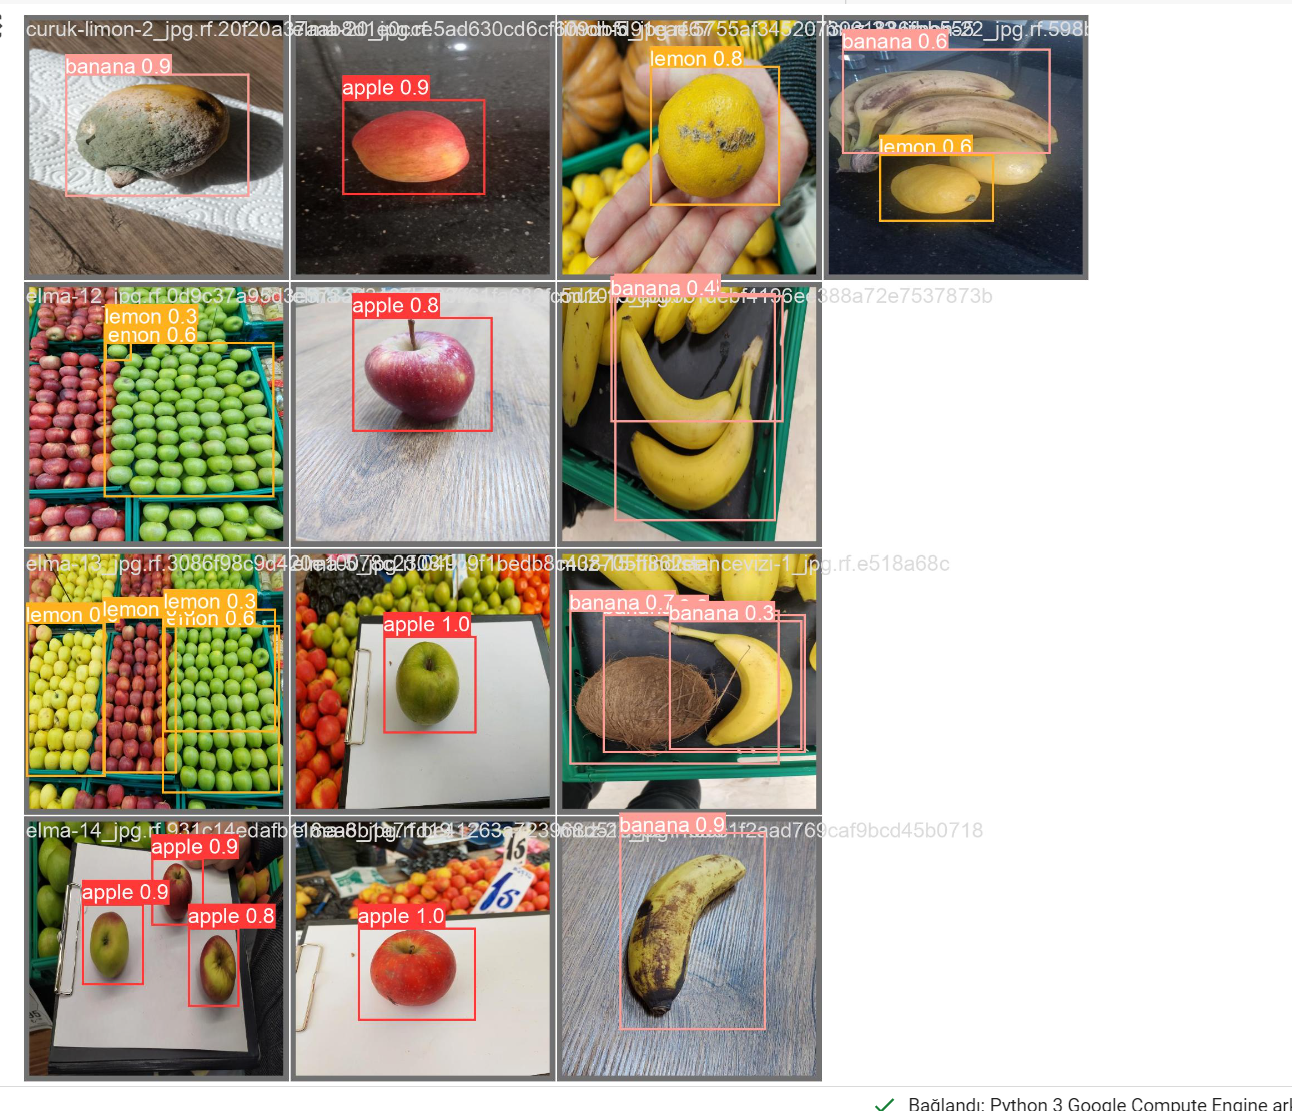
\includegraphics[width=\textwidth]{örnek2}
   		\caption{Nesne tespiti ile Güven Skoru}
   		
   	\end{figure}
   	 \textbf{Elma Sınıflandırması:} Model, farklı renklerdeki elma örneklerini genellikle doğru şekilde sınıflandıramadı. Kırmızı, yeşil ve sarı gibi farklı renklere sahip elmalara çoğunlukla doğru etiketler verilemedi.Model, bazı sarı renkli elma örneklerini limon olarak etiketledi. Bu durum, modelin renk bazında sınıflandırma yeteneğinde belirli bir hassasiyetsizlik olduğunu gösteriyor.
   	\newline
   	
   	\textbf{Muz ve Limon Sınıflandırması:} Sarı renkteki muz ve limon gibi meyveleri ayırt etme konusunda genel olarak iyi bir performans sergilemiştir. Model, muz ve limonları doğru şekilde sınıflandırdı ve genellikle bu meyveleri ayırt etmiştir. Ancak bazı durumlarda, özellikle çürük veya hasarlı limonların tanınmasında zorlanma yaşandı. Model, çürük limonları genellikle muz olarak sınıflandırdı.
   	
   	\subsection{ÇALIŞMA-2  WEBCAM İLE NESNE TANIMA }
   	Webcam'e bağlanarak gerçek zamanlı görüntü almak, nesne tanıma projemizin ilk adımıdır. Bu adımda, Spyder IDE'si kullanılarak Webcam'e bağlanma işlemi gerçekleştirilecektir.Webcam'den alınan görüntüleri daha sonra nesne tanıma algoritmalarıyla işlenecektir.
   	\newline
   	
   	OpenCV (Açık Kaynak Bilgisayar Görüntü İşleme Kütüphanesi): Webcam'e bağlanmak ve görüntü işlemek için kullanılacak olan temel kütüphanedir.
   	
\begin{figure}[!h]
	\centering
	\begin{subfigure}{0.45\textwidth}
		\centering
		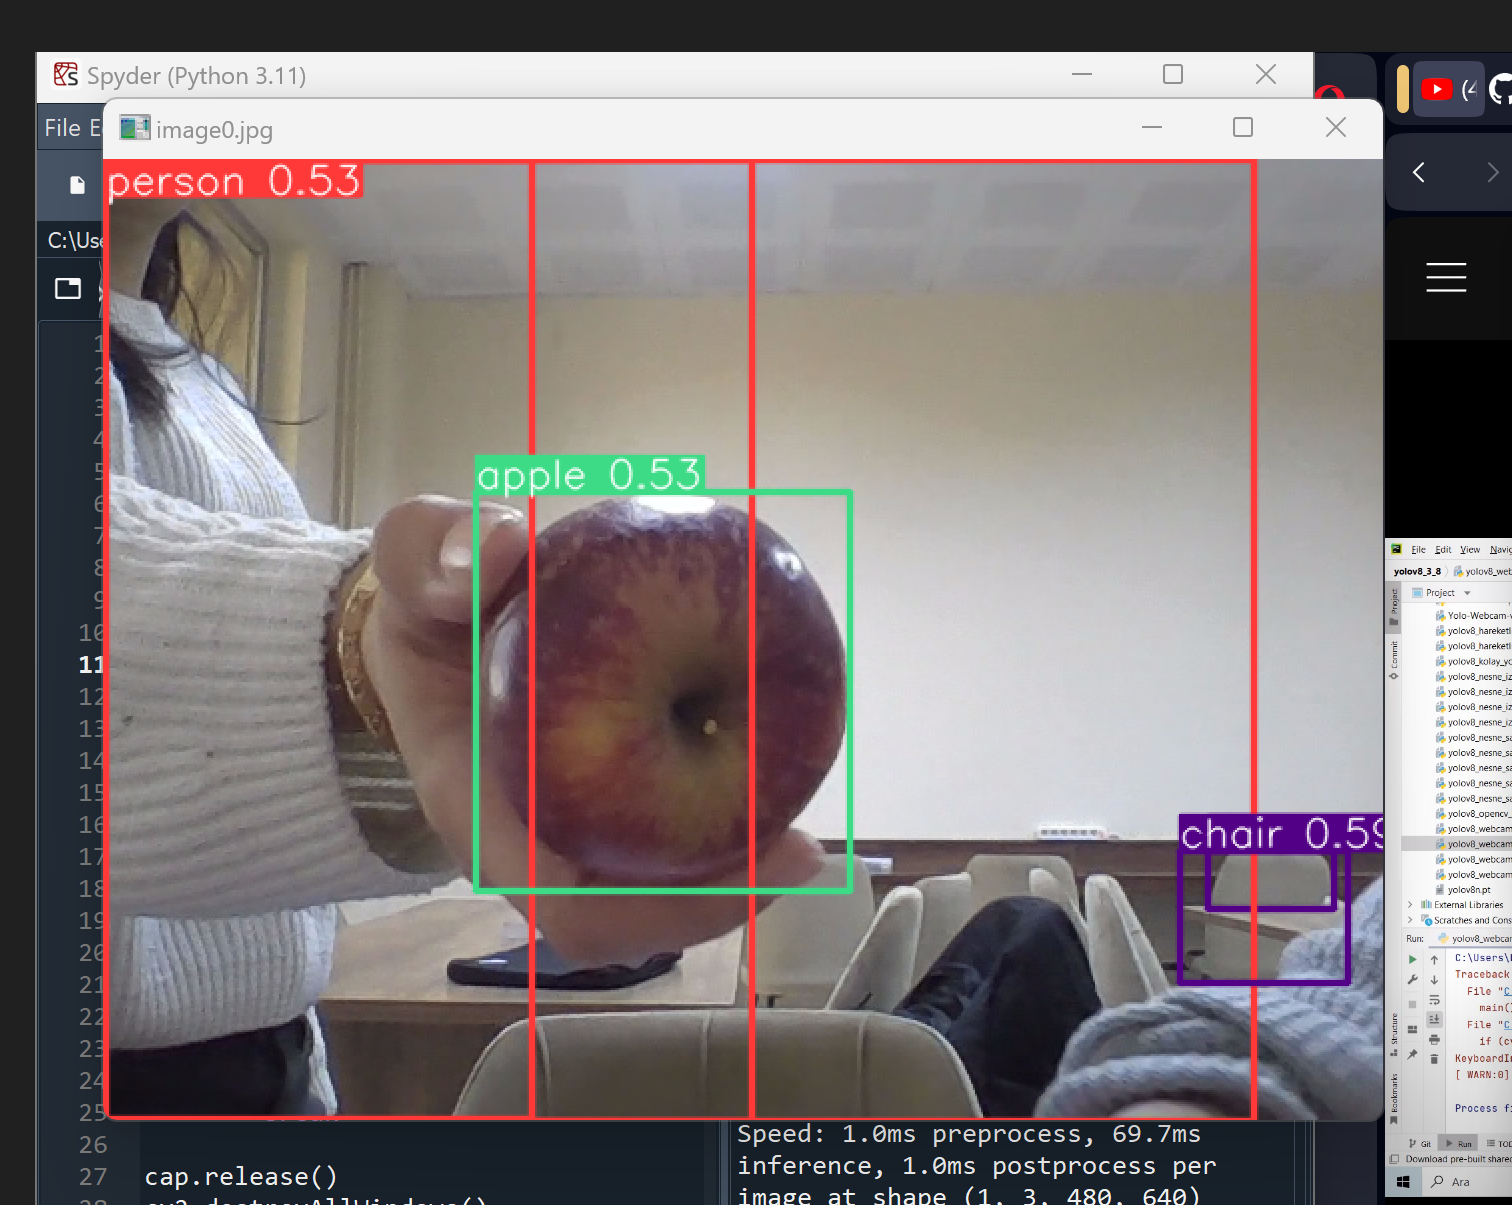
\includegraphics[width=1.16\linewidth]{nesne tanıma-1}
		\caption{Nesne Tanıma-1}
	\end{subfigure}
	\hfill
	\begin{subfigure}{0.45\textwidth}
		\centering
		\includegraphics[width=\linewidth]{domates-tanima}
		\caption{Nesne Tanıma-2}
	\end{subfigure}
	\caption{Nesne Tanıma Görselleri}
\end{figure}
\clearpage

\subsection{ÇALIŞMA-3  CANNY FONKSİYONU İLE KENAR TESPİTİ }

CANNY algoritması ile tespit edilen kenarların uzunluklarının hesaplanarak cismin boyutunun bulunması hedeflenmiştir. İlk olarak, farklı cisimlerde denenen algoritma sonrasında, meyvelerin tam sınırlarından çizilen bounding box'ların boyutunun bulunması ile meyvelerin yaklaşık boyutları belirlenmiştir. Bu süreçte, CANNY kenar tespiti algoritması ile meyvelerin sınırları belirlenmiş, ardından bu sınırlar kullanılarak bounding box'lar çizilmiştir. Çizilen bounding box'ların genişlik ve yükseklik değerleri hesaplanarak meyvelerin boyutları tahmin edilmiştir. Bu yöntem, meyvelerin yaklaşık boyutlarını belirlemek için pratik bir çözüm sunar ve farklı cisimlerde de uygulanabilirliği test edilmiştir.
\newline

	
\begin{figure}[!h] % Use [!h] to try to place the figure exactly here
	\centering
	\begin{subfigure}[t]{0.47\linewidth}
		\centering
		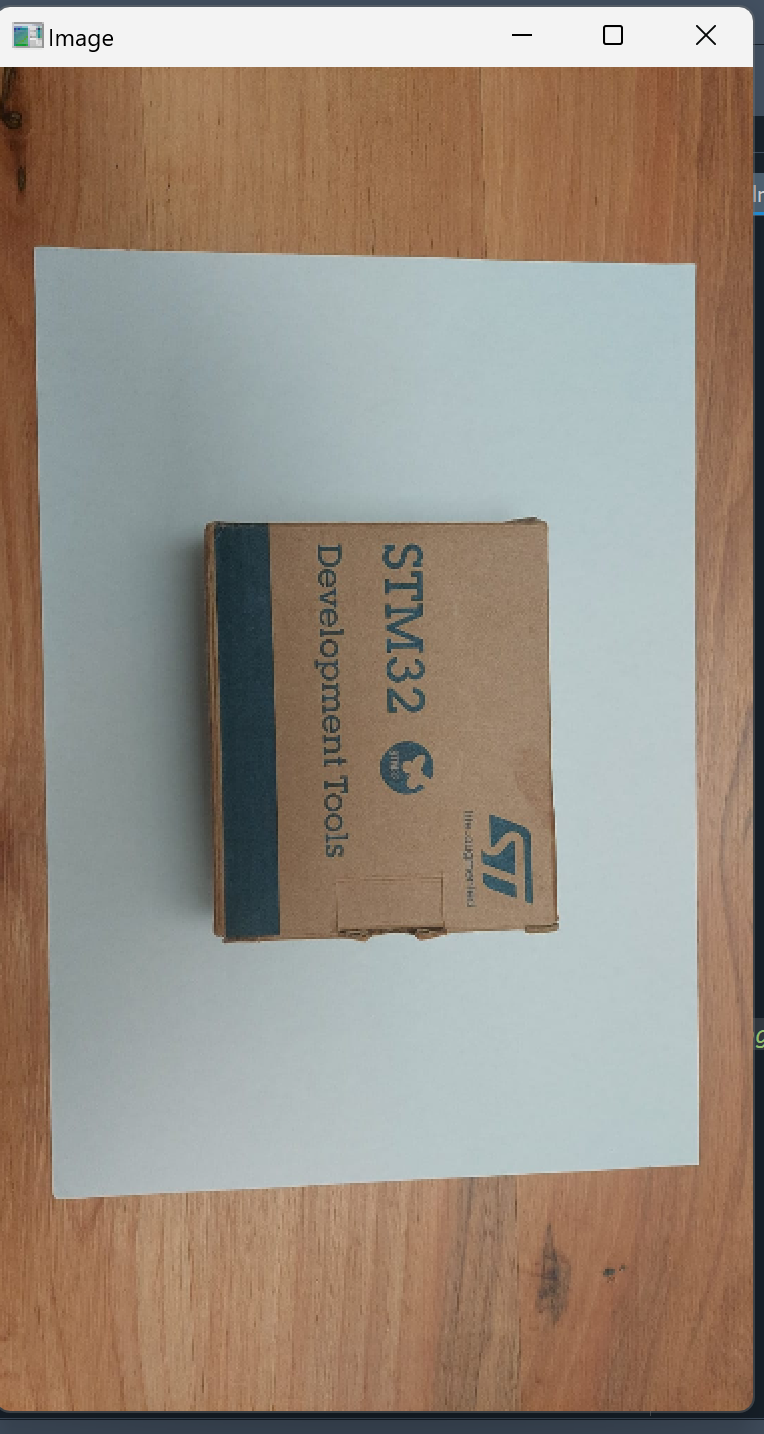
\includegraphics[width=\linewidth]{nesne-1-orijinal}
		\caption{Nesne'nin orjinal hali}
	\end{subfigure}\hfill
	\begin{subfigure}[t]{0.5\linewidth}
		\centering
		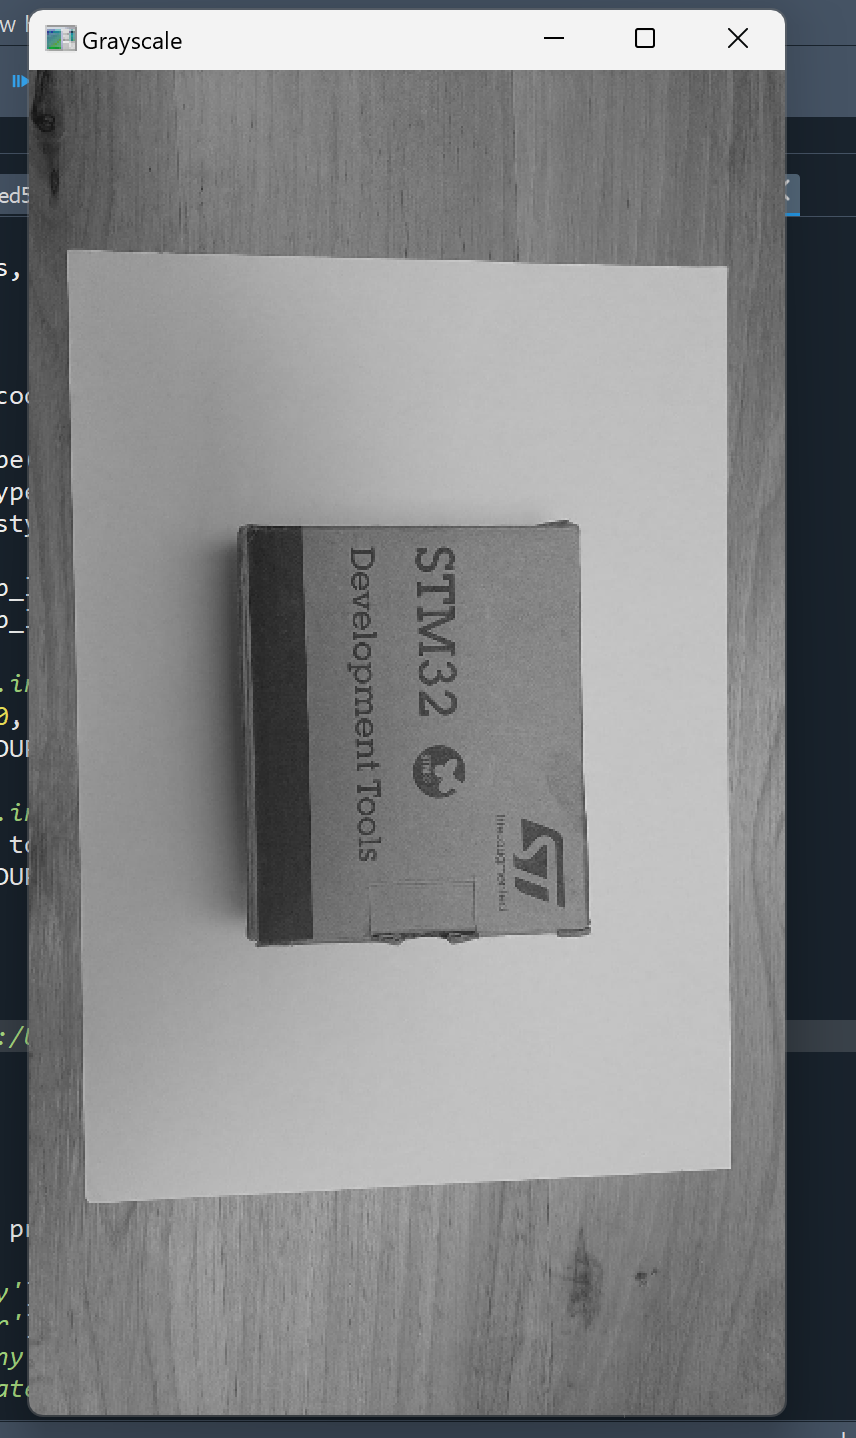
\includegraphics[width=\linewidth]{nesne-1-siyah}
		\caption{Siyah beyaz hali}
	\end{subfigure}

\end{figure}
	


\begin{landscape} % Rotating the page
	
	
\begin{figure}[!h] % Use [p] to place the figure on a separate page
		\centering
		
		\begin{subfigure}[t]{0.4\linewidth}
			\centering
			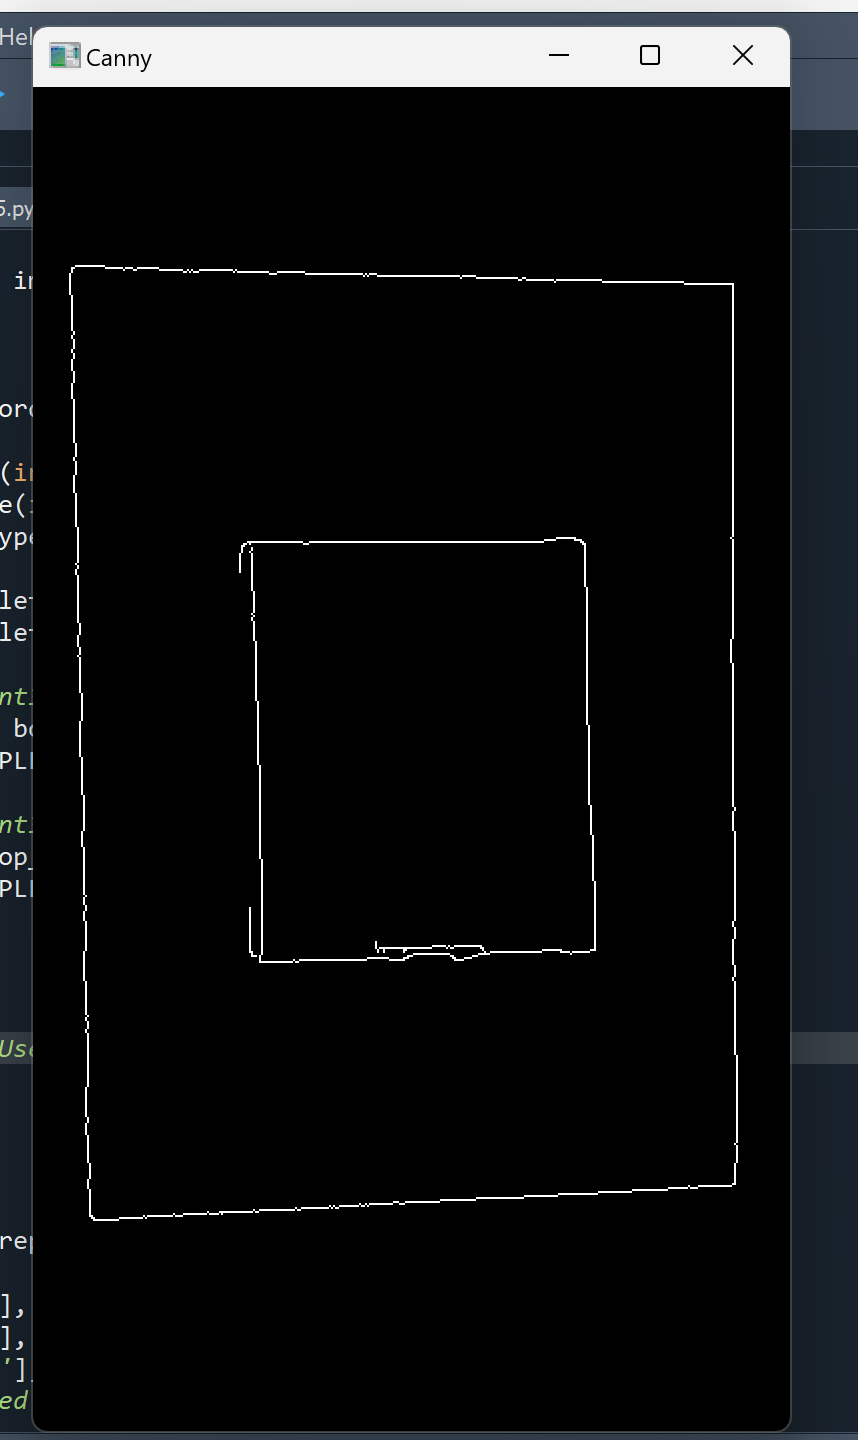
\includegraphics[width=\linewidth]{nesne-1-siyah-beyaz}
			\caption{Kenarlarının çizilmiş hali}
		\end{subfigure}\hfill
		\begin{subfigure}[t]{0.47\linewidth}
			\centering
			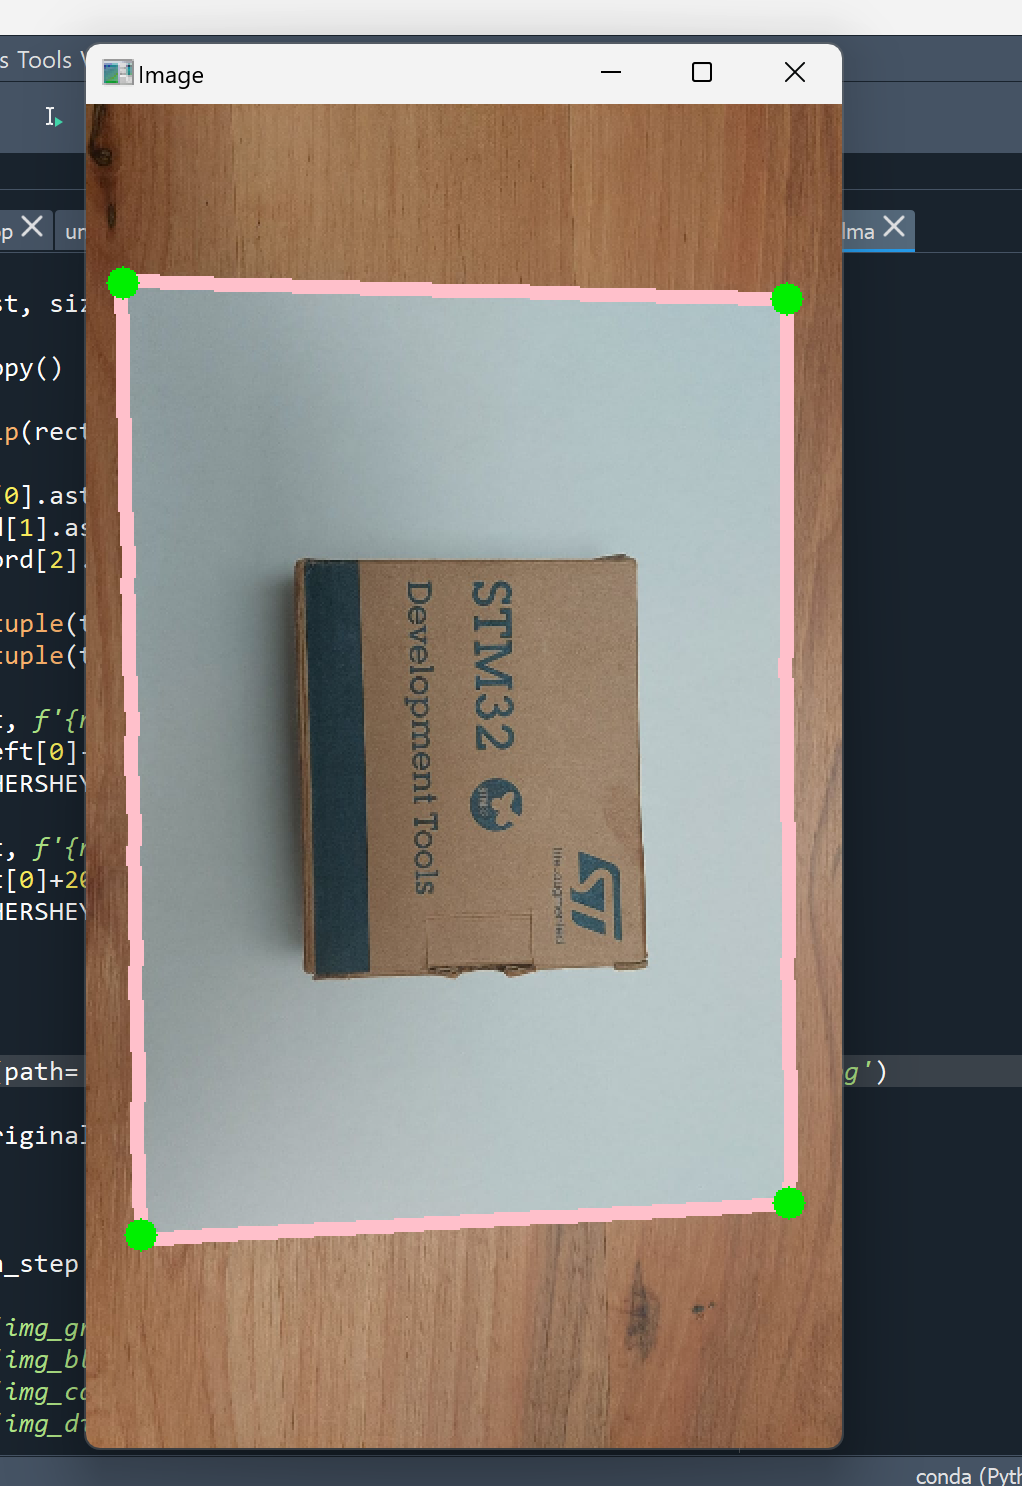
\includegraphics[width=\linewidth]{nesne-1-a4}
			\caption{Referansın kenarlarının çizilmesi}
		\end{subfigure}
\end{figure}
	
\end{landscape}

\begin{landscape} % Rotating the page
	
	
	\begin{figure}[!h] % Use [p] to place the figure on a separate page
		\centering
		
		\begin{subfigure}[t]{0.470\linewidth}
			\centering
			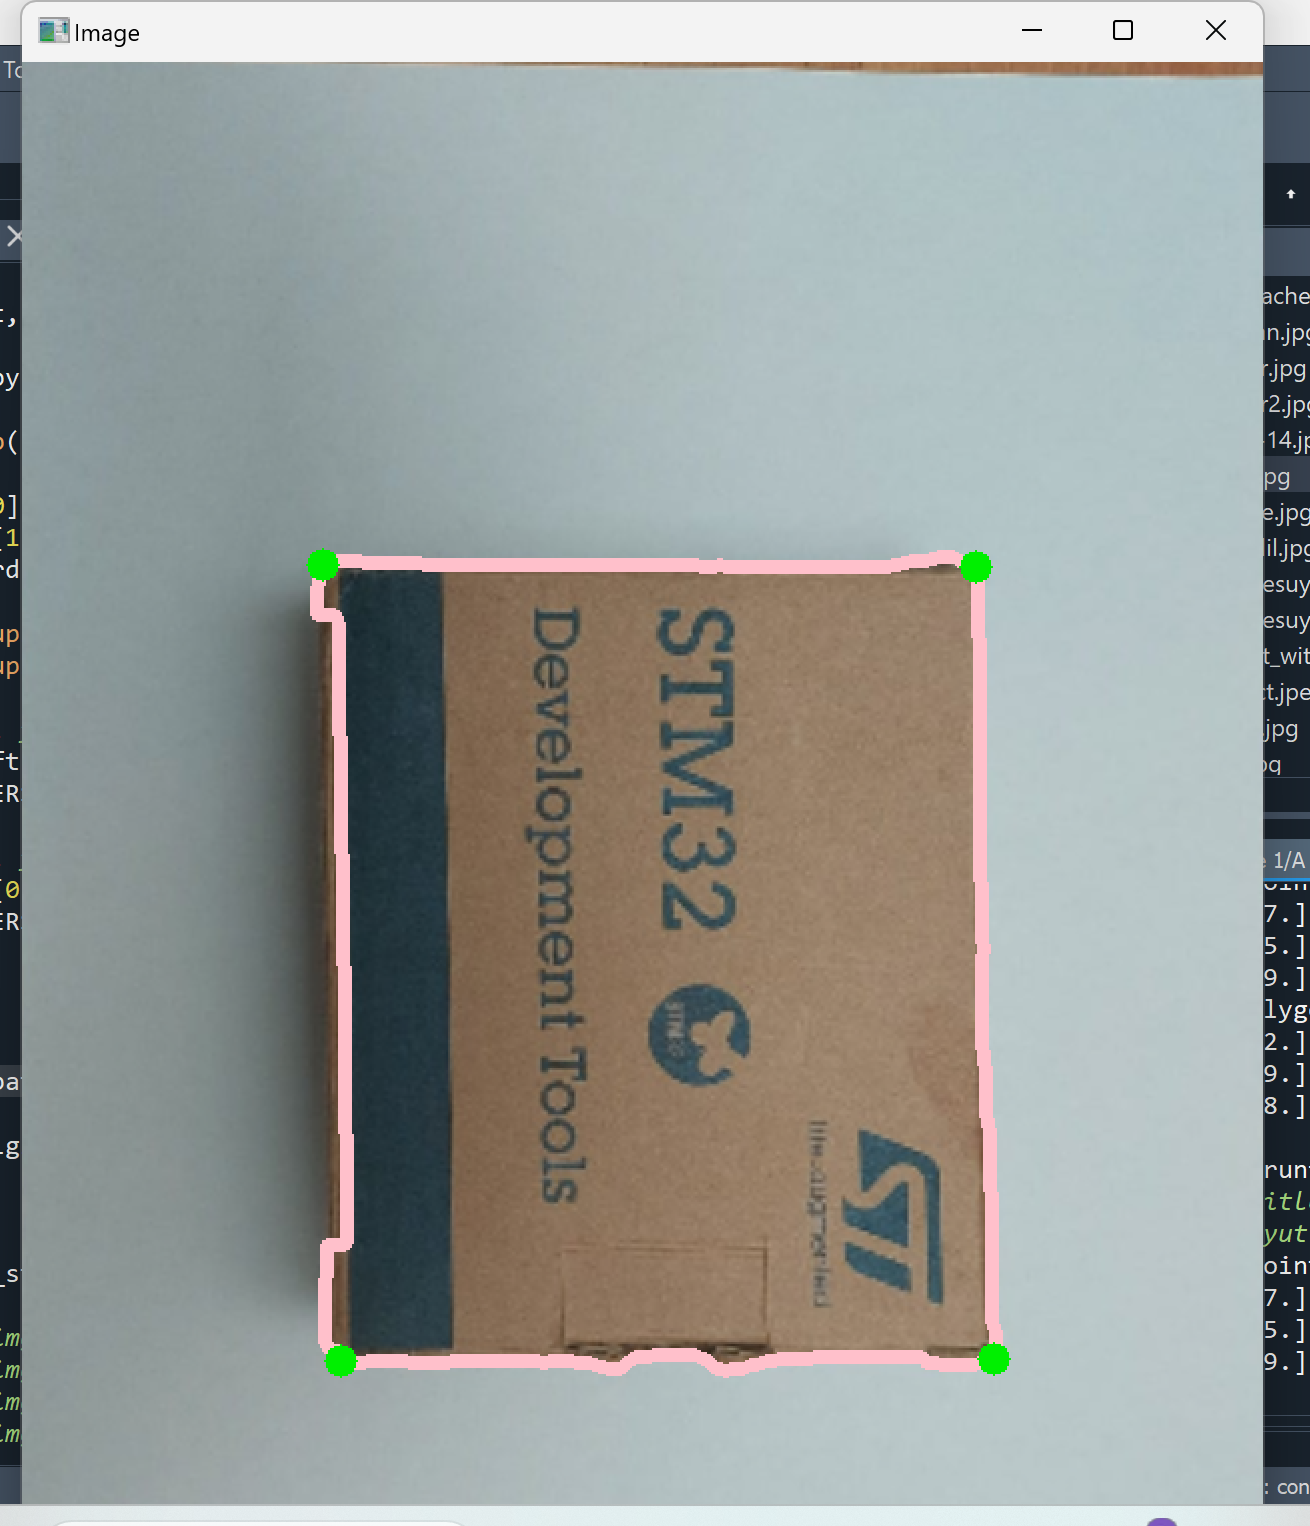
\includegraphics[width=\linewidth]{nesne-1-cerceve}
			\caption{Nesne'nin çevresinin çizilmesi}
		\end{subfigure}\hfill
		\begin{subfigure}[t]{0.49\linewidth}
			\centering
			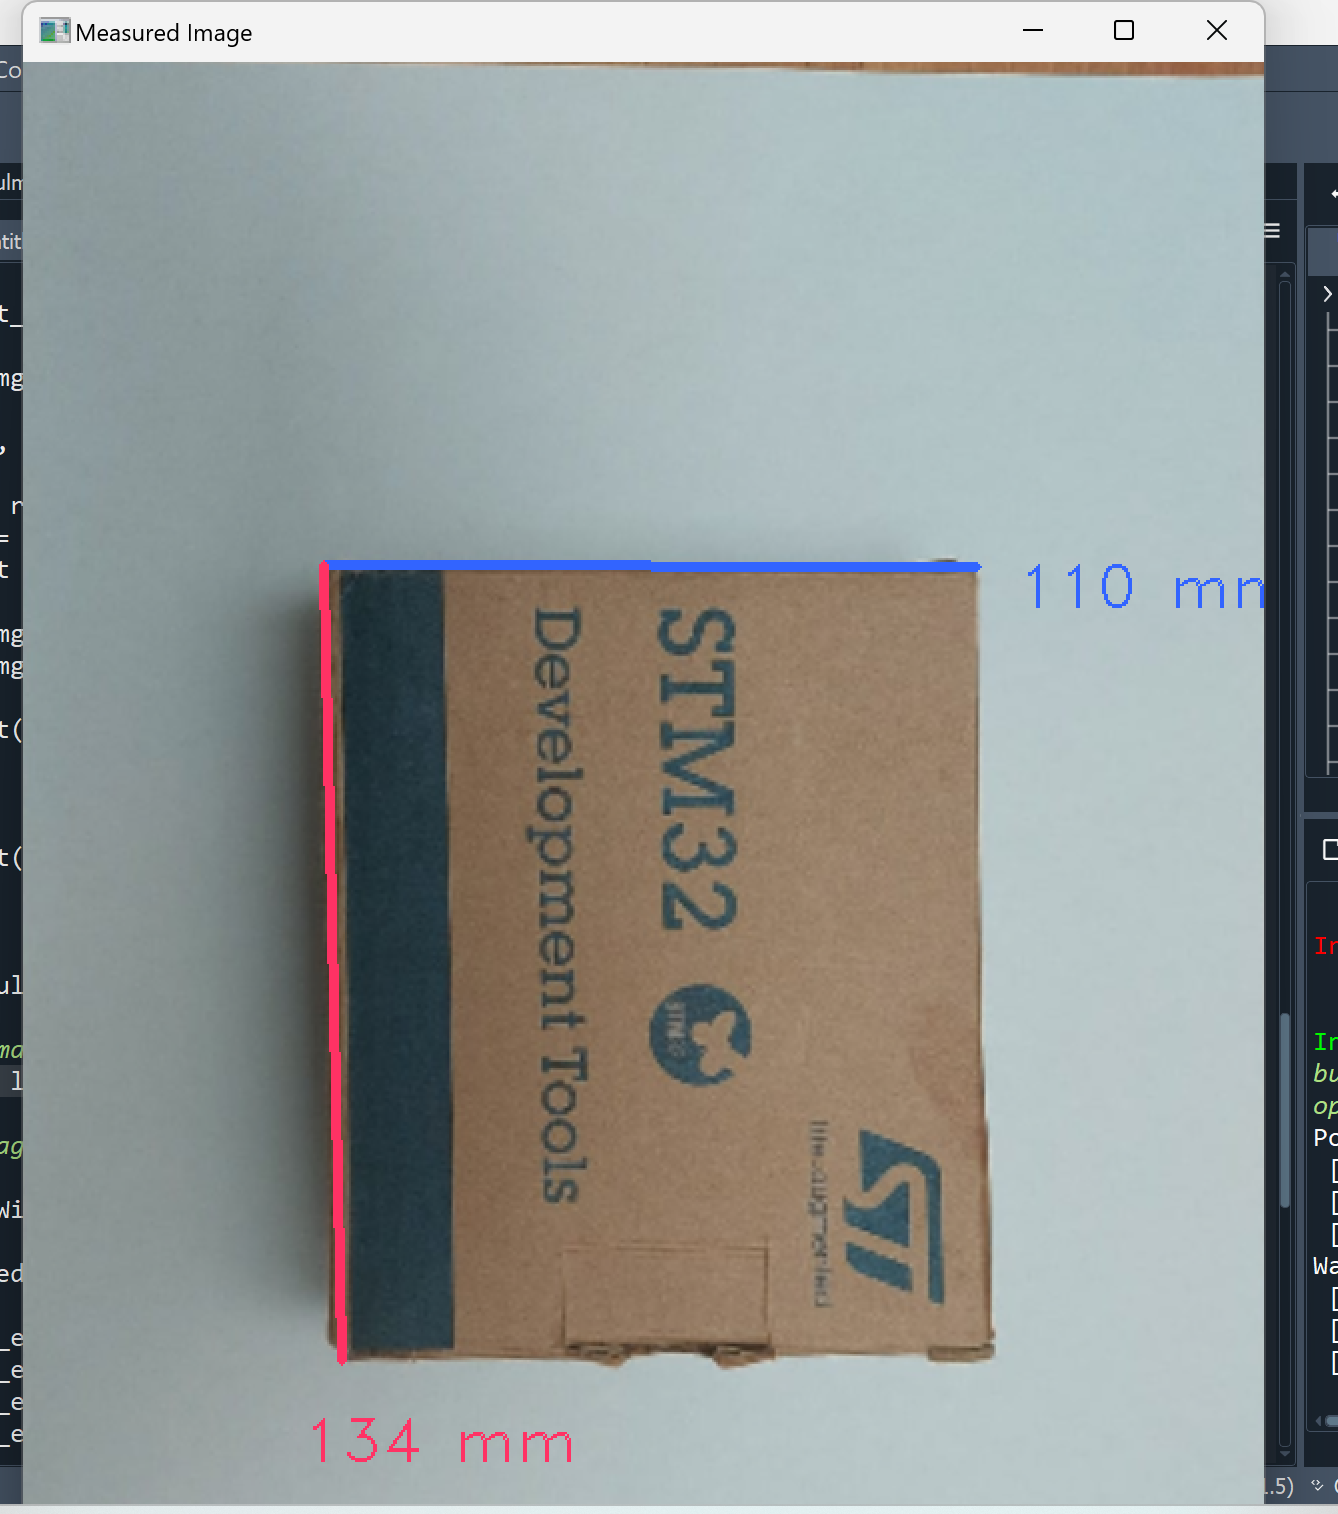
\includegraphics[width=\linewidth]{boyut-bulma-sonuc-1}
			\caption{Nesnenin Boyutları}
		\end{subfigure}
		
	\end{figure}
	
     \end{landscape}
     
  \subsection{Veri Seti Üzerinde Boyutlandırma Çalışmaları}
  Canny algortiması ile tespit edilen kenarlardan çizilen bouding box ile nesnenin yaklaşık boyutunun bulunması hedeflenmiştir.
 \vspace{0.2cm}

  	\begin{figure} [!h]
  		\centering
  	
  		\begin{subfigure}[t]{0.38\linewidth}
  			\centering
  			\includegraphics[width=\linewidth]{avakado}
  			\caption{Avokado Pixel Ölçümü}
  			\label{avakado}
  		\end{subfigure}\hfill
  		\begin{subfigure}[t]{0.36\linewidth}
  			\centering
  			\includegraphics[width=\linewidth]{biber2}
  			\caption{Biber Pixel Ölçümü}
  			\label{biber2}
  		\end{subfigure}
  		
  		\vspace{0.1cm} % Adjust vertical space between rows
  		
  		\begin{subfigure}[t]{0.38\linewidth}
  			\centering
  			\includegraphics[width=\linewidth]{biber-px-boyut}
  			\caption{Domates Pixel Ölçümü}
  			\label{biber}
  		\end{subfigure}\hfill
  		\begin{subfigure}[t]{0.38\linewidth}
  			\centering
  			\includegraphics[width=\linewidth]{cilek-boyut}
  			\caption{Çilek Pixel Ölçümü}
  			\label{cilek}
  		\end{subfigure}
  		\begin{subfigure}[t]{0.38\linewidth}
  			\centering
  			\includegraphics[width=\linewidth]{elma}
  			\caption{Elma Pixel Ölçümü}
  			\label{elma}
  		\end{subfigure}
  		

  		\caption{Pixel Ölçümleri}
  	\end{figure}
  	
  	 Şekil -\ref{avakado},-\ref{biber2},-\ref{cilek},-\ref{elma},-\ref{biber} de bulanıklaştırma yöntemi ile sınırları belirlenen cisim için tam kenarlarından geçen bouding box çizimi gösterilmektedir.Bouding box ile cisimlerin yaklaşık boyutu hesaplanmıştır.\cite{Nesne-Boyutlandırma}\cite{Nesne-Boyutlandırma-pixel}
  \clearpage
  \subsection{BaşParmak Oran Bulunması}
  \begin{figure}[!h]
  	\centering
  	\includegraphics[ width=0.5\textwidth]{Basparmak}
  	\caption{BaşParmak Oranı}
  	\label{basparmak}
  \end{figure}
  Şekil -\ref{basparmak} de isaret parmağının altın oranından yola çıkarak işaret parmağın pixel boyutunun altın oranına olan oranından başparmak için bir oran bulunmuştur.Bu oran cisimlerin gerçek boyutunu bulmada kullanılacaktır.
  \newline
  
  \subsection{El Boyutuna Oranla Gerçek Boyut Bulma}
  Bu kısımda önceden ayrı ayrı yapılan 2 projenin birleştirilip birlikte çalışması sağlanmıştır.Eldeki işaret parmağının referans olması için piksel boyutunun hesaplandığı proje ile cisimlerin tespit edilip piksel olarak uzunluk ve genişliğinin bulunduğu ve cismin ne olduğunun tespit edildiği projeler birleştirilmiştir.
  \vspace{0.2cm}


	\begin{figure}[!h] % Use [p] to place the figure on a separate page
	\centering
	
	\begin{subfigure}[t]{0.45\linewidth}
		\centering
		\includegraphics[width=\linewidth]{biber-2}
		\caption{Biber Pixel Ölçümü}
	\end{subfigure}\hfill
	\begin{subfigure}[t]{0.51\linewidth}
		\centering
		\includegraphics[width=\linewidth]{domates}
		\caption{Domates Pixel Ölçümü}
	\end{subfigure}
	 \vspace{0.4cm}
	
		\begin{subfigure}[t]{0.45\linewidth}
		\centering
		\includegraphics[width=\linewidth]{domates-2}
		\caption{Domates Pixel Ölçümü}
	\end{subfigure}
		\begin{subfigure}[t]{0.48\linewidth}
		\centering
		\includegraphics[width=\linewidth]{limon}
		\caption{Limon Pixel Ölçümü}
	\end{subfigure}
	\newline
	
	\caption{Cisimlerin Pixel Boyutları Ve El Tanınması}
\end{figure}
\clearpage


   \end{justify}
   \newpage
   
   
   \section{SONUÇ}	
   Bu çalışmada, webcam kamerası ile algılanan nesnelerin YOLO algoritması kullanılarak tespiti ve daha sonrasında MediaPipe ile el ölçümünden yola çıkarak gerçek ölçülerinin bulunması hedeflenmiştir. Yapılan işlemler sonucunda, nesnelerin boyutları piksel cinsinden bulunmuş ve bu sonuçlar el ölçüsü kullanılarak gerçek boyutlara dönüştürülmek üzere bir aşamaya getirilmiştir.
   \newline
   
   Nesne tanıma işlemi için YOLO algoritması kullanılarak başarılı bir şekilde nesneler tespit edilmiştir. Tespit edilen nesnelerin sınırları, bounding box kullanılarak belirlenmiş ve bu sınırlar içerisindeki nesnelerin yükseklik ve genişlik boyutları piksel cinsinden ölçülmüştür. Bu piksel ölçümleri, daha sonra MediaPipe kullanılarak el ölçümleri ile entegre edilmiştir.
   
   Bu entegrasyon, nesne boyutlarının doğru bir şekilde gerçek dünya ölçümlerine dönüştürülmesini sağlamayı amaçlamaktadır. Şu ana kadar, nesnelerin piksel cinsinden boyutları belirlenmiş ve el ölçüsü verileri ile oranlanarak gerçek boyutların bulunması aşamasına gelinmiştir. Son adım olarak, bu oranlama işlemi tamamlandığında, elde edilen sonuçlar sayesinde nesnelerin gerçek boyutları yüksek doğrulukla hesaplanabilecektir.
   \newline
   
   Sonuç olarak, bu çalışma, nesne tanıma ve boyut belirleme konularında önemli bir ilerleme kaydetmiş olup, uygulamanın son aşaması olan oranlama işlemi ile gerçek boyutların hesaplanmasına çok yakındır. Bu yaklaşım, çeşitli alanlarda pratik uygulamalar için kullanılabilir ve nesnelerin doğru boyutlarının tespit edilmesinde faydalı olabilir.
   
   \begin{justify}
   \end{justify}
   
	\bibliographystyle{plain}
	\bibliography{kaynakca}
\end{document}